\documentclass[12pt]{ociamthesis}  % default square logo 
%\documentclass[12pt,beltcrest]{ociamthesis} % use old belt crest logo
%\documentclass[12pt,shieldcrest]{ociamthesis} % use older shield crest logo

%load any additional packages
\usepackage{amssymb}
\usepackage{amsmath}
\usepackage{listings}
\usepackage{textcomp}
\usepackage{lmodern}
\usepackage{pdfpages}
\usepackage{url}

\lstset{language=Scala, upquote=true, columns=fullflexible, basicstyle=\ttfamily, keywordstyle=\bfseries, breaklines=true, breakatwhitespace=false}
%input macros (i.e. write your own macros file called mymacros.tex 
%and uncomment the next line)
%\include{mymacros}

%My shortcuts:
\newcommand{\R}{\mathcal{R}}
\newcommand{\K}{\mathbf{K}}
\newcommand{\coll}[2]{#1 \rightarrow #2}
\newcommand{\prim}[1]{\textrm{\textit{#1}}}
\newcommand{\OR}{\: | \:}
\newcommand{\Bag}[1]{\prim{Bag}[#1]}
\newcommand{\For}[2]{\textrm{for}(#1 \leftarrow #2)}
\newcommand{\If}[1]{\textrm{ if #1}}
\newcommand{\ForIf}[3]{\For{#1}{#2 \If #3}}
\newcommand{\Yield}[1]{\textrm{ yield } #1}
\newcommand{\YieldP}[2]{\Yield #1 \mapsto #2}
\newcommand{\Collect}[1]{\textrm{ collect } #1}
\newcommand{\proj}[2]{#1.\_#2}
\newcommand{\pair}[2]{\langle #1, #2 \rangle}
\newcommand{\Label}{\prim{Label}}
\newcommand{\String}{\prim{String}}
\newcommand{\Int}{\prim{Int}}
\newcommand{\Unit}{\prim{Unit}}
\newcommand{\vs}{\vspace{1em}}
\newcommand{\lin}[1]{\lstinline{#1}}
\newcommand{\G}{\Gamma}
\newcommand{\dX}{\delta_X}
\title{Efficient Processing of Nested Collections in Apache Spark}   %note \\[1ex] is a line break in the title

\author{Theodore Dickson}         %your name
\college{Worcester College}  %your college

%\renewcommand{\submittedtext}{change the default text here if needed}
\degree{MSc in Computer Science}     %the degree
\degreedate{September 2018}         %the degree date

%end the preamble and start the document
\begin{document}

%this baselineskip gives sufficient line spacing for an examiner to easily
%markup the thesis with comments
\baselineskip=18pt plus1pt

%set the number of sectioning levels that get number and appear in the contents
\setcounter{secnumdepth}{3}
\setcounter{tocdepth}{3}


\maketitle                  % create a title page from the preamble info
%%\include{dedication}        % include a dedication.tex file
%%\include{acknowlegements}   % include an acknowledgements.tex file
\begin{abstract}
Apache Spark is a parallel data processing framework with a generic collection API, allowing the distributed processing of any serialisable datatype. Though this allows the construction and processing of nested collections, severe performance issues are encountered when these nested collections exhibit skew due to the inability to distribute them among multiple worker nodes. Further, many nested queries are unable to be incrementalised efficiently. Attempts to rectify this often involve a technique called shredding, which decouples the nested collections from the main query and allows them to be distributed and updated separately. However, many of the shredding transformations proposed have limited scope in the queries to which they can be applied, and are not offered as programmatic tools which can automatically transform queries.

In this work we develop a variant of the Nested Relational Calculus (NRC) which supports a compositional and generic shredding transformation. We implement it with a Scala DSL, which allows NRC queries to be expressed with natural and minimal syntax. The DSL can shred and evaluate queries on local Scala collections, Spark RDDs and Spark DStreams, and is easily extensible to other data types. We also contribute several novel techniques for developing DSLs in Scala which are generally applicable to many similar tasks.

We obtain performance gains of up to [***] on shredded queries on Spark DStreams, although not all queries are sped up by shredding. We conclude that while shredding shows promise and this work contributes greatly to the ease of implementing such query transformations, further work would be necessary in order to enable shredding to be a worthwhile optimisation to integrate with Spark or other data processing frameworks.  
\end{abstract}          % include the abstract

\begin{romanpages}          % start roman page numbering
\tableofcontents            % generate and include a table of contents
%%\listoffigures              % generate and include a list of figures
\end{romanpages}            % end roman page numbering

%now include the files of latex for each of the chapters etc
\chapter{Introduction}

\section{Problem statement} {

Apache Spark \cite{spark} is an open-source framework for in-memory parallel processing of datasets. It utilises a cluster-computing architecture which transparently distributes data across many worker nodes in a network. Since its initial release in 2014 it has quickly become one of the most popular frameworks for large-scale data analysis, owing largely to its user-friendly functional APIs (offered in Scala, Python, R and SQL) and impressive out-of-the-box performance. A number of domain-specific libraries, such as for machine learning and graph processing, have further enabled its wide adoption in industry.

Although Spark can transform collections of arbitrary types, it can exhibit severe performance problems when processing nested data (i.e. data with inner collections). Data of this type is commonplace, for example nested formats such as JSON and XML, or graphs in the adjacency list format. In particular, distributed processing of such data where the nested collections have skewed cardinalities leads to load imbalance amongst the machines in the cluster. At best, load imbalance causes inefficient use of resources. At worst, machines with the heaviest loads can run out of memory, causing slowdowns when results spill to the disk, and eventually total program failure when disk space runs out as well. Crucially, heavily skewed data is surprisingly common, owing to the power-law dynamics which govern many naturally occurring phenomena, especially social networks and other graph-like structures.

Additionally, although Spark offers powerful abstractions for processing streamed data, many queries involving nested collections do not incrementalise well. That is to say, it is not possible to process only the new batch and update the output with the latest result. Instead, with each new batch of data in the stream, the entire output must be recomputed.

Spark unfortunately does not offer any tools to deal with these performance issues. Users must manually rewrite affected queries in order to flatten their inputs and/or outputs. However, this process is time-consuming and error prone, not least because many datasets are more naturally reasoned about as containing nested collections. The popularity of the aforementioned nested data formats is testament to this.

}

\section{Motivating example} {

To demonstrate this issue, consider the following scenario. A streaming music service allows listeners to rate tracks as they listen to them, with either a like (+1) or a dislike (-1). These ratings are accessed via an \lin{RDD[(User,Track,Date,Int)]}, where each row represents a single integer rating given to a track by a user on a given date. Additionally there is an \lin{RDD[(Track,Artist)]} associating tracks to artists. The streaming services wishes to compute a new dataset which contains, for each artist, the aggregate ratings for each track on each date. They wish to store this data in nested form so that it can efficiently provide the results in JSON form for an endpoint in the service's public API. Therefore they must compute a new RDD with one row per artist, where each has a nested collection which associates each of the artist's tracks to a further inner collection of aggregate ratings for each date. This RDD would thus have type \lin{RDD[(Artist,Map[Track,Map[Date,Int]])]}. Figure \ref{exsparkquery} describes a Spark query which would be a standard way to to compute this.

\begin{figure}
\begin{lstlisting}
val ratings: RDD[(User,Track,Date,Int)]
val trackArtists: RDD[(Track,Artist)]

//calculate total ratings for each track on each date,
//by grouping by track and then aggregating the
//ratings for each date
val ratingsByDate: RDD[(Track,Map[Date,Int])] =
  ratings.groupBy(_._2)
    .map { case (track,ratings) =>
      (track,
        ratings.map { case (_,_,date,value) => (date,value) }
          .reduceByKey(_ + _)
      )
  }

//calculate the set of ratings by date for each artist,
//by joining trackArtists to the grouped ratings
//and then grouping by artist
val artistRatings: RDD[(Artist,Map[Track,Map[Date,Int]])] =
  ratingsByDate.join(trackArtists)
    .map { case (track,(ratings,artist)) => (artist,(track,ratings)) }
    .groupBy(_._1)
    .mapValues { case rows =>
      rows.map { case (_,(track,ratingsByDate)) => (track,ratingsByDate) } toMap
    }
\end{lstlisting}
\caption{Spark query to compute the aggregate track ratings by date for each artist.}
\label{exsparkquery}
\end{figure}

Firstly, this query is likely to exhibit severe load-balancing issues. This is because the grouping of the ratings by track will aggregate every rating for a given track into a single row. And further, the grouping by artist will then aggregate every track rating for that artist into a single row. However, due to the natural power-law dynamics of many social phenomena such as music popularity \cite{musicpowerlaw}, a small number of tracks will represent a large proportion of the ratings, and an even smaller number of artists will represent a large number of these tracks. In particular, there will probably be some artists with hundreds of thousands or even millions of track ratings, while others have hundreds or fewer. Thus, the workers which happen to contain such rows will be more likely to run out of memory, potentially crashing the query, and even if they don't, the imbalance will lead to some workers finishing further processing of the ratings far sooner than others, which is an inefficient use of resources.

Secondly, this query cannot be \textit{efficiently incrementalised}. This means that its results cannot be updated with an efficient \textit{union} operation, given a new batch of data, without reprocessing the original output in any way. To demonstrate this, suppose that the music service instead wishes to calculate an up-to-date version of this dataset every hour, by processing an \lstinline{RDD} of the ratings for the last hour and combining this with the previous version. That is, suppose we have:
\vs\begin{lstlisting}
val oldArtistRatings: RDD[(Artist,Map[Track,Map[Date,Int]])]
val ratingsDelta: RDD[(Track,Date,Int)]
\end{lstlisting}\vs
and then we calculate the above query \textit{trackRatingsByArtist} just for the latest ratings, producing:
\vs\begin{lstlisting}
val artistRatingsDelta: RDD[(Artist,Map[Track,Map[Date,Int]])]
\end{lstlisting}\vs
Then the RDD:
\vs\begin{lstlisting}
val newArtistRatings = oldArtistRatings.union(artistRatingsDelta)
\end{lstlisting}\vs
is not the correctly up-to-date version. It will include duplicate entries for each artist appearing in both the old version and the latest ratings. Further, even if we were to group by the artists and reduce, the reduction
of the nested maps would be quite expensive, and writing such logic manually would be error-prone. 
}


\section{Shredding} {

Our approach is to transform such queries using a process called \textit{shredding}, which solves the two root causes of the problem. First, Spark only parallelises processing at the top-level, and thus has no mechanism for distributing inner collections, which is the cause of load imbalance.  Second, the construction of nested collections does not benefit from the algebraic property of distributivity, as we will see in Section \ref{nrcexprsection}, which is what prevents efficient incrementalisation.

Shredding does this by pinpointing the places in a query in which nested collections are constructed, and instead replaces them by unique defining labels. Hence, the principal output of a shredded query is flat - that is, it contains no nested collections. Along with the flat output, the shredding transformation additionally produces a \textit{shredding context}. This is a set of queries which compute dictionaries defining the inner collections associated to each label. As these dictionaries are decoupled from the main query, they can be implemented in such a way that the definitions of the labels can in fact be distributed as well as efficiently updated.

In our simple example above, the principal output would be an \lstinline{RDD[(Artist,Label1)]}, thus the outermost nested collection is simply replaced by a single label. The shredding context would contain two dictionaries. The first would define \lin{Label1}, and so would be of type \lin{Dictionary[Label1,Map[Track,Label2]]} (implementation of the dictionaries is discussed in Chapter \ref{evaluation}). Since there is another collection nested within this one, we can see that the definition itself contains a label. This would in turn be defined in a second dictionary of type \lin{Dictionary[Label2,Map[Date,Int]]}. In this way, shredding is a compositional, generic transformation which can decouple and distribute inner collections at arbitrary levels of nesting within a query. Chapter \ref{nrc} describes the rich algebraic structure that enables this.

However, this shredded output comes with a tradeoff. When the nested collections defined by the dictionaries are needed, there is a cost to looking them up. Whether the tradeoff is beneficial overall will depend on the structure of the input data, the type of query and how the output is consumed. In data with only minor skew, the lookup cost may not be worth a relatively small load-balancing benefit, whereas when the skew is more severe, it is more likely to have a measurable performance benefit.

It will also depend on whether the entire nested output is needed, or just part of it. In the music service scenario for example, if each API request only needs the nested output for a small number of artists, the lookup costs in the system will be very small compared to the load-balancing benefits.

With regard to incrementalised (or streamed) queries, the benefit of this tradeoff will be highly dependent on how frequently the output is consumed. For example, if the query is consumed very infrequently compared to how often it is updated, the more efficient updates may counteract even a very high lookup cost.

\subsection{Automating shredding} {
In this work, we use a variant of the nested relational calculus (NRC) and shredding transformation introduced in \cite{draftpaper}. While it was shown that certain queries can be processed significantly faster using shredding, the shredding transformation was applied manually. Although this demonstrated the validity of the approach, and provided a strict algorithmic process for manual query-rewriting, it does not truly solve the problem.

Therefore our goal is to implement the automatic shredding of queries without sacrificing the performance benefits demonstrated in \cite{draftpaper}. We aim to do this by providing a domain-specific language (DSL) in which users can express NRC queries with natural syntax, and then automatically evaluate them in Spark using the shredding transformation.
}

\section{Related work} {
The problems presented by large and/or skewed nested collections in parallel environments have attracted significant attention, but efforts to tackle the issue have focussed largely on the way in which they are stored. An algorithm proposed by Dremel \cite{melnik2010dremel} (the record shredding and assembly algorithm) describes a columnar format which effectively stores arbitrarily nested collections in shredded form. This is the basis of the Parquet format \cite{parquet} developed by Apache for use in the Hadoop ecosystem, including with Spark.

However, the Spark data processing model itself does not encompass any shredding primitives, and thus shredded records are re-assembled before any processing can occur. Thus shredding transformations for queries offer the possibility of operating on shredded data without the need for reassembly. That said, many of the popular proposals, such as \cite{grust2009ferry} and \cite{lindley2012row}, are aimed at underpinning language-integrated query systems rather than supporting the translation of arbitrary nested queries. To this end they are geared towards generating SQL queries and make use of SQL-specific primitives which is not compatible with our objective of translating Spark queries.

Further, those that do propose more general, algebraic systems for translating queries, such as Van den Bussche \cite{van2001simulation}, which shows that is is possible to evaluate nested queries over sets of flat queries, do not propose implementations of these proposals and so shredding remains relatively inaccessible to users of frameworks such as Spark. Therefore our goal of an end-to-end system for query shredding, encompassing both a proven algebraic transformation and a fully developed Scala implementation which integrates with Spark, would be a significant contribution to the field.		
}



}


\section{Contributions} {
The main contributions of this work are as follows:

\begin{itemize}
\item{We provide a Scala DSL which allows users to easily write NRC queries with natural syntax. Queries written in this way can be automatically evaluated, with or without the shredding transformation applied, with the full runtime safety guarantees of the Scala compiler. This DSL works with both local collections and Spark collections, and is easily extensible to other frameworks thanks to a clean, modular design based largely on the typeclass pattern.}
\item{We introduce an updated version of the NRC which enabled the automatic evaluation of queries in Spark, by replacing constructs which proved hard to translate to valid Spark code.}
\item{We present a novel and generally applicable technique for inferring the types of variables within a Scala DSL at compile-time, thus avoiding the need to manually tag them. }
\item{\textit{(summary of performance benefits)}}
\end{itemize}
}

\section{Structure of the text} {
The rest of the report proceeds as follows. In Chapter \ref{nrc}, we introduce the variant of the NRC used in this work, and define the shredding transformation on queries written in this calculus. In Chapter \ref{dsl}, we describe the basic implementation of the DSL - both how we appropriately represent queries and how we use advanced Scala features to allow these queries to be generated with user-friendly syntax. Chapter \ref{evaluation} demonstrates how we evaluate these queries, both with and without shredding, and in Chapter \ref{incrementalisation} we extend the DSL to incrementally evaluate queries as well. In Chapter \ref{results} we provide some experimental results and discuss their significance. Finally, in Chapter \ref{conclusion} we provide some concluding remarks including possible directions for future work.
}
\chapter{Nested Relational Calculus} \label{nrc}

In this chapter we explain the variant of the nested relational calculus used in this work.
First we explain how its semantics allow arbitrary nesting of collections, and introduce the core algebraic operators, showing how they enable a wide range of queries. Then we introduce some syntactic constructions which allow us to more naturally express nested queries. We explain the two forms that nested queries can take (key-nested and value-nested), and why the former is preferable semantically but not efficiently parallelised or incrementalised. Next we introduce the delta expressions for each operator, and show that while most operators incrementalise efficiently due to their algebraic properties, others must be recomputed with each update. Finally we provide a full description of the shredding transformation, and show how it allows us to simulate the semantics of a single key-nested query with a set of value-nested queries, thus retaining the performance benefits of value-nesting.


\section{Type system} {

In order to apply the shredding operation outlined in the previous chapter, we introduce a variant of the nested relational calculus which uses \textit{generalised multiset semantics}. As opposed to a regular multiset, or \textit{bag}, in which each element in a set is associated with an integer value, in our generalised multiset semantics we model collections by mappings $ \coll{\K}{\R} $ where values can be of any type which admits a ring structure $ (\R,0_\R,+_\R,-_\R,1_\R,*_\R) $. In the following we will show the two key properties of these semantics. Firstly, that they admit nesting of collections to arbitrary depth, and secondly, that they give rise to the potential for efficient incrementalisation and parallelisation since the majority of the operators we will introduce are distributive ring operations.

Figure \ref{nrctypes} formally describes the type system that enables these semantics, using an inductive definition.

\begin{figure}
\begin{equation*}
\begin{aligned}
&\R := \prim{Int} \OR \prim{Bool} \OR \R \times  \R \OR \coll{\K}{\R} \\
&\K := \prim{Dom} \OR  [\R]  \OR \prim{Label} \\
\end{aligned}
\qquad
\begin{aligned}
\end{aligned}
\end{equation*}
\caption{The type system of the NRC}
\label{nrctypes}
\end{figure}

It will also be useful to introduce the notation $\Bag{\K} := \coll{\K}{\prim{Int}}$, for collections with integer multiplicity.

\subsection{Ring types} {
The base cases of our ring type are the integers and the booleans. Integers admit the ring structure $(\mathbb{Z},0,+,-,1,*)$, and booleans the structure $(\mathbb{B}, false,OR,NOT,true,AND)$. Note that it is trivial to extend this calculus to other primitive types admitting a ring structure, such as the real numbers, but for brevity we omit these. 

The first of our inductive cases is the product type $\R \times \R$. A product of two ring types $\R_1$ and $\R_2$ trivially admits a ring structure by pairing the 0 and 1 elements and applying the operations of $\R_1$ and $\R_2$ element-wise. Although in practice we will be able to use tuples of any arity, in this formalism we only define operations for a pair, as higher arities are isomorphic to nesting products within the second element.

The second and crucial inductive case is the collection type $\coll{\K}{\R}$, which itself admits a ring structure in which $\R$'s operations are applied element-wise over the key space $\K$. For example, if we have two collections $X: \coll{\K}{\R}$ and $Y: \coll{\K}{\R}$ then:

\begin{equation*}
\begin{split}
& (X+Y)(k)  = X(k) +_\R Y(k) \\
& (X*Y)(k) = X(k) *_\R Y(k)
\end{split}
\end{equation*}

If $\R$ is an $\prim{Int}$, so that $X,Y: \Bag{\K}$, then we can see that $+$ corresponds to bag union. We can also see that $*$ is thus join-like when applied to collections - a key will only have non-zero value in the resulting collection if it has non-zero value in each of $X$ and $Y$. In this way, we equate the existence of a key with it having non-zero value. Hence the zero element $0_{\coll{\K}{\R}}$, which is the empty collection, is equivalent to the collection where every $k \in \K$ is mapped to the zero element $0_R$. This underlines the incrementalisation potential of this algebraic framework, as it means deletions can be modelled with updates to keys with negative value.

Thus, can use collections themselves as multiplicities. For example, a collection of type $\coll{\K_1}{(\coll{\K_2}{\R})}$ associates a collection of type $\coll{\K_2}{\R}$ to each key of type ${\K_1}$. This is what we call \textit{value} or \textit{ring} nesting and is the first way to obtain nested collections.

\subsection{Key types} {

For keys, the base types are the $\prim{Dom}$ types. These are the types of the active domain of the database. When using Apache Spark for example, this constitutes all serializable Scala data types. In a typical relational database this would be much more restricted, to types such as INT, FLOAT, VARCHAR, TIMESTAMP, and so on. 

The type $[\R]$ (the boxed ring type) offers ring types for use as keys while retaining the view of their ring structure, thus marking the places where shredding can be performed. For example, a collection of type $\coll{(\K_1,[\coll{\K_2}{\R}])}{\prim{Int}}$ maps a pair of two key types, $\K_1$ and the boxed ring type, $[\coll{\K_2}{\R}]$ to a multiplicity of $\prim{Int}$ type. This is what we call \textit{key nesting}. 

The $\prim{Label}$ type represents places we have applied shredding, in order to replace key-nested collections with labels. For example, in a query which produces a result of type  $\coll{(\K_1,[\coll{\K_2}{\R}])}{\prim{Int}}$, we would expect shredding to instead produce a result of type 
$\coll{(\K_1,\prim{Label})}{\prim{Int}}$, along with a dictionary of type $\coll{\prim{Label}}{(\coll{\K_2}{\R})}$. Note that both of these types do not contain key-nested collections. Instead our dictionary uses value-nesting. This will be crucial to how we efficiently incrementalise such shredded queries.

}

\section{Expressions} \label{nrcexprsection}

Figure \ref{nrcexprs} introduces the constructions that define the valid expressions in our calculus. In this section we explain these and discuss their algebraic properties.

\begin{figure}
\begin{equation*}
\begin{split}
k := \ & c \OR x \OR \langle k_1, k_2 \rangle \OR \proj{k}{i} \\ \\
r := \ & c \OR X \OR \langle r_1, r_2 \rangle \OR \proj{r}{i} \OR \\
& r_1 + r_2 \OR -r \OR r_1 \ast r_2 \OR r_1 \cdot r_2 \OR \\
& join(r_1,r_2) \OR sum(r) \OR p(k) \OR \\
& sng(k,r) \OR \{ x => r \} \OR group(r)
\end{split}
\end{equation*}
\caption{Valid expressions in the NRC.}
\label{nrcexprs}
\end{figure}

\subsection{Ring expressions} {
The base expressions of ring type are constants and input collections, denoted by $c$ and $X$ respectively. Constants will be of $\prim{Int}$ or $\prim{Bool}$ type in this restricted formalism, but in practice can be of any numeric type or other primitive type admitting a ring structure. Input collections are datasets of type $\coll{\K}{\R}$, where $\K$ is any valid key type and $\R$ any valid ring type. For example, in our motivating example, the input collection \textit{ratings} is of type $\coll{(User \times Track \times Date)}{\prim{Int}}$. We also have a standard tupling operator denoted by $\langle , \rangle$ and can project such product types using the notation $\proj{r}{i}$.

Next we have $+$, $-$, and $\ast$, the algebraic operators defined by the ring structure of $\R$. It will be important when discussing incrementalisation and parallelisation to note that  $\ast$ is distributive with respect to $+$:
\[
a*(b + c) = a*b + a*c.
\]

The dot product ($\cdot$) is a generalised multiplication operator which accepts any two arguments of ring type. It is defined using $*$ as follows:
\begin{equation*}
\begin{split}
& \textrm{If } X: \prim{Int}, \ Y: \prim{Int}\textrm{, then } X \cdot Y = X * Y \\ \\
& \textrm{If } X: \coll{\K}{\R}, \ Y: \prim{Int}\textrm{, then } X \cdot Y : \coll{\K}{\R \cdot \prim{Int}}, \\
& (X \cdot Y)(k) = X(k) \cdot Y\textrm{, for all }k: \K \\ \\
& \textrm{If } X: \coll{\K_1}{\R_1}, \ Y: \coll{\K_2}{\R_2}\textrm{, then } X \cdot Y : \coll{\langle \K_1, \K_2 \rangle}{\R_1 \cdot \R_2} \\
& (X \cdot Y)(\langle k_1, k_2 \rangle) = X(k_1) \cdot Y(k_2)\textrm{, for all }k_1,k_2: \K
\end{split}
\end{equation*}
This operation can natively implement certain useful operations. For example, the dot product of a $\Bag{\K_1}$ and a $\Bag{\K_2}$ produces their cartesian product.

The dot product is distributive:
\vs\begin{equation*}
\begin{split}
& \textrm{If } X: \prim{Int}, \ Y: \prim{Int}\textrm, \ Z: \Int: \\
&X \cdot (Y + Z) = X * (Y + Z) = X*Y + X*Z = X \cdot Y + X \cdot Z \\ \\
& \textrm{If } X: \coll{\K}{\R}, \ Y: \prim{Int}, \ Z: \Int: \\
& (X \cdot (Y+Z))(k) = X(k) \cdot (Y+Z) = X(k) \cdot Y + X(k) \cdot Z = (X \cdot Y)(k) + (X \cdot Z)(k) \\ \\
& \textrm{If } X: \coll{\K_1}{\R_1}, \ Y: \coll{\K_2}{\R_2}, \ Z: \coll{\K_2}{\R_2} \\
& (X \cdot (Y+Z))(\langle k_1, k_2 \rangle) = X(k_1) \cdot (Y+Z)(k_2) = X(k_1) \cdot Y(K_2) + X(k_1) \cdot Z(k_2) \\
&= (X \cdot Y)(k_1) + (X \cdot Z)(k_2) 
\end{split}
\end{equation*}
It also allows us to extend the native ring multiplication operation to collections of the same key type but differing ring types, by defining the output value of each key as the dot product of the values of the key in each input collection:
\begin{equation*}
\begin{split}
& X: \coll{\K}{\R_1}, \ Y: \coll{\K}{\R_2} \\
& X * Y : \coll{\K}{\R_1 \cdot \R_2} \\
& (X*Y)(k) = X(k) \cdot Y(k)
\end{split}
\end{equation*}
We will see in \ref{forcomp} how this extension to multiplication allows us to define a for-comprehension construct with very natural semantics.

As previously mentioned, the $*$ operator can be described as join-like. However, even with this generalisation, it is not general enough to model many useful joins since it joins on the entire key. Thus we introduce a separate join operator, which only operates on collections, and joins only on the first element of a product-typed key. It is defined as follows:
\begin{equation*}
\begin{split}
& X: \coll{(\K,\K_1)}{\R_1},  Y: \coll{(\K,\K_2)}{\R_2} \\
& join(X, Y): \coll{(\K, (\K_1,\K_2))}{\R_1 \cdot \R_2} \\
& join(X, Y)(\langle k, \langle k_1, k_2 \rangle \rangle) = X(\langle k, k_1 \rangle) \cdot Y(\langle k, k_2 \rangle)
\end{split}
\end{equation*}
Thus, a key $\langle k, \langle k_1, k_2 \rangle \rangle$ will only be non-zero in the output if $\langle k, k_1 \rangle$ is non-zero in $X$ and $\langle k, k_2 \rangle$ is non-zero in $Y$. Equivalently, there will be a key  $\langle k, \langle k_1, k_2 \rangle \rangle$ in the output for every pair of keys $\langle k, k_1 \rangle \in X$ and $\langle k', k_2 \rangle \in Y$ such that $k == k'$. Hence, it models an inner join on the first element of the key. It is general enough to model all inner joins if we restructure the elements of a higher arity key as a pair where the element(s) we wish to join on constitute the first element of the key and the others are nested within the second element. 

\noindent The $join$ operator is also distributive:
\begin{equation*}
\begin{split}
&X: \coll{(\K,\K_1)}{\R_1},  \ Y: \coll{(\K,\K_2)}{\R_2}, \ Z: \coll{(\K,\K_2)}{\R_2} \\
&join(X,Y+Z)(\pair{k}{\pair{k_1}{k_2}}) = X(\pair{k}{k_1}) \cdot (Y+Z)(\pair{k}{k_2}) \\
&=X(\pair{k}{k_1}) \cdot Y(\pair{k}{k_2}) + X(\pair{k}{k_1}) \cdot Z(\pair{k}{k_2}) \\
&=join(X,Y)(\pair{k}{\pair{k_1}{k_2}}) + join(X,Z)(\pair{k}{\pair{k_1}{k_2}})
\end{split}
\end{equation*}

The sum operator is another which will be used in the for-comprehension construct, and is defined as follows: 
\begin{equation*}
\begin{split}
 & X: \coll{\K}{\R} \\
 & sum(X): \R \\
 & sum(X) = \sum_{k: K} X(k)
\end{split}
\end{equation*}
It is only defined for collection types, and, for example, when applied to a bag returns its aggregate count.
 
\vs The predicate operator $p(k)$ encapsulates any function accepting a key and returning a boolean. We will see how it enables us to do things such as filter collections.
 
\vs The \textit{singleton} constructor is $sng$. With $k: \K$ and $r: \R$, $sng(k,r)$ constructs a collection of type $\coll{\K}{\R}$ with the single element $k  \mapsto r$. We will see how this combines with our for-comprehension to more generally transform collections.
 
\vs The infinite mapping $\{x => r\}$ allows us to express functions from key types to value types as collections of infinite domain, where the key is a variable expression $x$ and the value is a ring expression $r$ which may use the variables introduced in $x$. When such an expression is multiplied with a finite collection, the variable expression is bound to each of the keys in the finite collection in order to produce a concrete result.

The following example shows us how this allows transformations of finite collections:

\noindent Let $k_1,k_2: K$ be variables. Let $X: \Bag{\K \times \K}$. Let $p(\langle k_1, k_2 \rangle) = k_1 == k_2$ be the predicate comparing $k_1$ and $k_2$ for equality. \\
Let $Y = X * \{\langle k_1, k_2 \rangle => p(\langle k_1, k_2 \rangle)\}$. \\ Applying the definition of *, and assuming $k_1,k_2$ are in the domain of $X$: \\
\begin{equation*}
\begin{split}
Y(\langle k_1, k_2 \rangle) &= X(\pair{k_1}{k_2}) \cdot 1 = X(\pair{k_1}{k_2})\textrm{, if } k_1 == k_2 \\
&= X(\pair{k_1}{k_2}) \cdot 0 = 0\textrm{, otherwise}
\end{split}
\end{equation*}
Hence $Y$ is X filtered to only those keys whose first and second elements are equal.

\vs The last ring-typed construct is group, and is the operator which constructs key-nested collections. It is defined on collections with keys of pair type, as follows:
\begin{equation*}
\begin{split}
&X: \coll{(\K_1 \times \K_2)}{\R} \\
&group(X): \coll{(\K_1 \times [\coll{\K_2}{\R}])}{\prim{Bool}} \\
&group(X)(\pair{k_1}{k_2'}) = true \iff k_2' = \sum_{(\pair{k_1'}{k_2} \mapsto r) \in X : \ k_1' = k_1} {\{k_2 \mapsto r\}} 
\end{split}
\end{equation*}
This creates a key in the output for each unique first element of the key in the input. These keys are paired with the boxed collection of all of the second elements they appear with in the input. In this way it is a grouping of the input by the first element of the key. For example:
\begin{equation*}
\begin{split}
&X: \Bag{\prim{String}\times \prim{String}} \\
&X = \{(a,b) \mapsto 1, (a, c) \mapsto 2, (b,d) \mapsto 3\} \\
&group(X) = \{\langle a, \{b \mapsto 1, c \mapsto 2\} \rangle \mapsto true, \langle b, \{d \mapsto 3 \} \rangle \mapsto true \}
\end{split}
\end{equation*}
This key-nested representation offers an important semantic benefit. It allows us to keep track of keys of type $\K_1$ whose nested collections become empty upon updates to the inputs of the query. Using the example above, suppose we receive an update to $X$:
\begin{equation*}
\dX = \{(\pair{b}{d} \mapsto -3\}
\end{equation*}
This translates to updating the key-nested collection $\pair{b}{\{d \mapsto 3\}}$:
\begin{equation*}
 \pair{b}{\{d \mapsto -3, d \mapsto 3\}} = \pair{b}{\{\}}
 \end{equation*}
However the entry $\pair{b}{\{\}} \mapsto true$ remains in the output, indicating that the inner collection keyed by $b$ exists but is empty.
Letting $group^v(X)$ be the value-nested representation of $group(X)$:
\begin{equation*}
group^v(X) = \{a \mapsto \{b \mapsto 1, c  \mapsto 2\}, b \mapsto \{d \mapsto 3\}\}
\end{equation*}
When we update this with $\{b \mapsto \{d \mapsto 3\}\}$, we get:
\begin{equation*}
group^v(X) = \{a \mapsto \{b \mapsto 1, c  \mapsto 2\}, b \mapsto \{d \mapsto 0\}\} = \{a \mapsto \{b \mapsto 1, c  \mapsto 2\}\}
\end{equation*}
And so $b$ disappears from the top-level of our output entirely. 

\subsection{Key expressions} {
The base key expressions are either constants, denoted $c$, or variables, denoted $x$, which are strictly those introduced as the keys of an infinite mapping. As with ring expressions, we also have tupling and projection. 
}

\section{For-comprehension syntax} { \label{forcomp}
In this section we introduce several variants of a familiar syntactic construction, the for-comprehension, which will allow many queries to be written more naturally.

Let $X$ be a finite collection of type $\coll{\K}{\R}$, $r_1$ be a ring expression of type $\R_1$, and $x$ be a variable of type $\K$. Our basic for-comprehension syntax is thus defined as:
\begin{equation*}
\For{x}{X} \Collect{r_1} := sum(X * \{x => r_1\})
\end{equation*}
It is helpful to think of this as iterating over the key-value pairs $\pair{k}{r}$ in $X$, calculating the value of $r_1$ for each key $k$, and aggregating the result of multiplying this with $r$. For example, with $X: \Bag{\Int}$, the query:
\begin{equation*} 
\For{x}{X} \Collect{x > 2} = sum(X * \{x => x > 2\})
\end{equation*}
calculates the aggregate count of the keys in $X$ which are greater than 2, since:
\begin{equation*}
\begin{split}
(X*\{x => x > 2\})(y) &= X(y)*true = X(y)\textrm{, if } y > 2 \\
 &= X(y)*false = 0\textrm{, otherwise.}
\end{split}
\end{equation*}
We now add a variant of this which enables filtering collections with a natural syntax. With $p(x)$ a predicate expression:
\begin{equation*}
\ForIf{x}{X}{p(x)} \Collect{x > 2} := sum(X * \{x => r_1 \cdot p(x) \})
\end{equation*}
Hence, we can instead write the above query as:
\begin{equation*}
\begin{split}
\ForIf{x}{X}{x > 2} \Collect{1} &= sum(X * \{x => 1 \cdot (x > 2) \}) \\
&=sum(X * \{x => x > 2) \}
\end{split}
\end{equation*}
These examples are quite limited in that they are only aggregations of a collection $X$. In order to transform $X$ more generally, we can use the singleton constructor. For example, consider the following query:
\begin{equation*}
\begin{split}
&X: \coll{(\K_1 \times \K_2)}{\R} \\
&Y = \For{\pair{k_1}{k_2}}{X} \Collect{sng(\pair{k_2}{k_1}, 1)}
\end{split}
\end{equation*}
Then $Y$ is $X$ but with the pairs reversed. To see how this works, let's examine the translation of $Y$ into basic syntax: 
\[ Y = sum(X*\{\pair{k_1}{k_2} => sng(\pair{k_2}{k_1},1)\}) \]
The inner expression $X*\{\pair{k_1}{k_2} => sng(\pair{k_2}{k_1},1)\}$ iterates over $X$ and and maps each key $\pair{k_1}{k_2}$ to its original value, multiplied by $sng(\pair{k_2}{k_1},1)$. Thus, suppose $X = \{\pair{a}{b} \mapsto 1, \pair{c}{d} \mapsto 2\}$, then:
\begin{equation*}
X*\{\pair{k_1}{k_2} => sng(\pair{k_2}{k_1},1)\} = \{(a,b) \mapsto \{(b,a) \mapsto 1\}, (c,d) \mapsto \{(d,c) \mapsto 2\}\}
\end{equation*}
Then the sum outside this aggregates all of the values via bag union, to produce the single flat collection:
\begin{equation*}
\{(b,a) \mapsto 1, (d,c) \mapsto 2\}
\end{equation*}
Which is indeed $X$ with the elements of the keys reversed. We encapsulate this construct with the following variant of our for-comprehension: 
\begin{equation*}
\begin{split}
\ForIf{x}{X}{p(x)} \Yield{k \mapsto r} &:= \ForIf{x}{X}{p(x)} \Collect{sng(k,r)} \\
& \ = sum(X * \{x => sng(k,r \cdot p(x)) \})
\end{split}
\end{equation*}
The $r$ is optional and defaults to 1. Thus, we can write the above query to reverse the elements in a product-type key as:
\[\For{\pair{k_1}{k_2}}{X} \Yield{\pair{k_2}{k_1}}\]
This is clearly a very natural syntax with which to manipulate collections corresponding to similar syntax in many programming languages.

\subsection{Example query} \label{examplequery}

With the for-comprehension syntax, we can now express the query from the motivating example. The \lin{ratings} RDD can be represented by a $\Bag{\prim{User} \times \prim{Track} \times \prim{Date}}$, where the $\Int$ values are the rating given to the track by the given user on the given date. The association table is a $\Bag{\prim{Track} \times \prim{Artist}}$, where the values are all 1. Then the query is:
\begin{equation*}
\begin{split}
&trackRatings = group(\For{\langle u,t,d \rangle}{ratings} \Yield{\pair{t}{d}}) \\
&artistTrackRatingsFlat = join(trackArtists,trackRatingsByDate) \\
&artistTrackRatings = group( \For{\langle t,\langle a,rs \rangle \rangle}{artistTrackRatingsFlat} \Yield{\langle a, \langle t,rs \rangle \rangle})
\end{split}
\end{equation*}

Here, $trackRatings$ first projects the ratings to just the track and date, thus aggregating for each such pair the total rating across all users. It then groups this by track, returning a $\coll{(\prim{Track} \times [\Bag{\prim{Date}}])}{\prim{Bool}}$, representing the pairing of each track with its aggregate rating for each date. Then this is joined with the track association table, which adds the artist to each key, producing a $\coll{(\prim{Track} \times (Artist \times [\Bag{\prim{Date}}]))}{\prim{Bool}}$. Finally, $artistTrackRatings$ reorders the elements of the key with a for/yield so that the artist is the first element, and applies group in order to produce the final
$\coll{(\prim{Artist} \times [\coll{(\prim{Track} \times [\Bag{\prim{Date}]})}{\prim{Bool}}])}{\prim{Bool}}$. This collection will have one key per artist, where the artist is the first element, and the collection of ratings for each track on each day is nested within the second element.
}

\section{Restricted construction of key-nested collections}
The $group$ operator is the only way in this calculus to construct key-nested collections. We recognise that this is quite restrictive. In fact, in \cite{draftpaper}, the variant of the NRC used does not include this construct, but instead uses a more general construct $toK$ which boxes arbitrary sub-queries of ring type. Unfortunately, although this allows for a more general query language, the queries written in this way proved highly impractical to implement within Spark. For example, to express the grouping of a collection $X: \Bag{\K_1 \times \K_2}$ by the first element of the key, the following query would be used:
\begin{equation*}
\begin{split}
&\For{\pair{k_1}{k_2}}{X} \\
&\Yield{\pair{k_1}{toK(\ForIf{\pair{k_1'}{k_2'}}{X}{k_1 == k_1'} \Yield k_2')}}
\end{split}
\end{equation*}
Here, the logic to group is expressed by a nested iteration, filtered by a predicate to test for equality of the inner key with the outer key.
The naive way to implement the evaluation of such a query would lead to physically performing this nested iteration, which is clearly very inefficient compared to implementing it with a grouping primitive. Further, in Spark, nested iteration of RDDs is not supported at all.
Thus, without a dedicated optimiser to examine these queries and detect when nested iterations filtered by predicated correspond to grouping or other primitives, it is not possible evaluate such queries in Spark.

Hence it was decided to forego this operator in favour of the explicit $group$ operator which can be directly evaluated using the \lin{groupBy} method on an RDD, as we will see in Chapter \ref{evaluation}.
Despite this, we will see in Chapter \ref{results} that even with this restriction we are still able to express a wide range of complex queries. 

}

\section{Incremental updates to queries} { \label{deltas}



In this section we introduce \textit{delta expressions}, or expressions which compute the update to a query given an update to its inputs. For example, if we have some expression $r$ with an input collection $X$, and receive an update $\delta X$ for $X$ such that the new value of $X$ is $X^{new} = X + \delta X$, the delta expression $\delta_X(r)$ is the expression such that $r^{new}$ = $r + d_X(r)$.

\begin{figure}
\begin{equation*}
\begin{aligned}
&\delta_X(c) = 0 \qquad \delta_X(X) = \Delta X \qquad \delta_X(Y) = 0\\
&\delta_X(\pair{r_1}{r_2}) = \pair{\delta_X(r_1)}{\delta_X(r_2)} \qquad \delta_X(\proj{r}{i}) = \proj{\delta_X(r)}{i}\\
&\delta_X(r_1 + r_2) = \delta_X(r_1) + \delta_X(r_2) \qquad \delta_X(-r) = -\delta_X(r)\\
&\delta_X(r_1 * r_2) = \delta_X(r_1)*r_2 + r_1*\delta_X(r_2) + \delta_X(r_1) * \delta_X(r_2) \\
&\delta_X(r_1 \cdot r_2) = \delta_X(r_1) \cdot r_2 + r_1 \cdot \delta_X(r_2) + \delta_X(r_1) \cdot \delta_X(r_2) \\
&\delta_X(join(r_1,r_2)) = join(\delta_X(r_1),r_2) + join(r_1,\delta_X(r_2)) + join(\delta_X(r_1),\delta_X(r_2)) \\
&\delta_X(sum(r)) = sum(\delta_X(r)) \qquad \delta_X(\{x => r\}) = \{x => \delta_X(r)\} \\
&\delta_X(sng(k,r)) = sng(e^{new},r)  + sng(e^{new},\delta_X(r)) - sng(e^{old},r) \\
&\delta_X(group(r)) = group(r + \delta_X(r)) - group(r)
\end{aligned}
\qquad
\end{equation*}
\caption{Delta derivation rules for NRC expressions.}
\label{deltaexprs}
\end{figure}

Figure \ref{deltaexprs} shows these expressions. The fact that the updates are modelled with addition allows us to exploit the algebraic properties of the operators to derive efficient delta expressions in the majority of cases. For example, we exploit the linearity of $+$ to derive the delta rule:
\[\delta_X(r_1 + r_2) = \delta_X(r_1) + \delta_X(r_2)\]
since: 
\[r_1^{new} + r_2^{new} = (r1 + \delta_X(r_1)) + (r2 + \delta_X(r_2)) = (r_1 + r_2) + (\delta_X(r_1) + \delta_X(r_2))\]
Linearity is similarly used for $-$ and $sum$. These rules are efficient because they do not depend at all on $X$, only $\delta X$.

\vs The slightly more complicated rules for multiplication, the dot product, and the join operator are a result of their distributivity. We illustrate the derivation of the rule for multiplication below:
\begin{equation*}
\begin{split}
(r_1 + \delta_X(r_1))*(r_2 + \delta_X(r_2)) &= (r_1 + \delta_X(r_1))*r_2 + (r_1 + \delta_X(r_1))*\delta_X(r_2) \\
&= r_1*r_2 + \delta_X(r_1)*r_2 + r_1*\delta_X(r_2) + \delta_X(r_1) * \delta_X(r_2) \\
\implies \delta_X(r_1*r_2) &= \delta_X(r_1)*r_2 + r_1*\delta_X(r_2) + \delta_X(r_1) * \delta_X(r_2)
\end{split}
\end{equation*}
This derivation is also valid for the dot product and join operator as it only uses the distributive property which they all share. While these rules are not quite as efficient as the rules for the linear operators, they are still much more efficient than re-computing. This is because the terms that do depend on an input collection, e.g. $\delta_X(r_1) * r_2$, will constitute a join in practice between an update and only one of the input collections. Since the updates are in general small compared to the size of the input collections, these joins will be much more efficient that the cost of the original join between the two input collections.

\vs Unfortunately, we can see that the expressions for $sng$ and $group$ are not efficient - they do require recomputation. In the case of $sng$, this is because if the key-typed argument is affected by the update, the singleton collection must be fully reconstructed. However, if it is unaffected by the update, so that $e^{new} = e^{old} = e$, the delta expression simplifies as follows:
\begin{equation*}
\begin{split}
sng(e^{new},r) + sng(e^{new},\delta_X(r)) - sng(e^{old},r) &= sng(e,r) + sng(e,\delta_X(r)) - sng(e,r) \\
&= sng(e,\delta_X(r))
\end{split}
\end{equation*}
In practice, usage of $sng$ will largely be confined to the for/yield construction where the yielded key is a variable expression, and so will be unaffected by updates to input collections. 

For $group$, the delta expression is not efficient because the construction of key-nested collections is fundamentally not distributive or linear. Thus, the only way to compute an updated output is to compute the updated input, apply $group$ to this, and substract the previous output. However, we will see in the next section how shredding removes the need for this recomputation by converting the construction of a key-nested collection into the construction of value-nested collection, which does indeed distribute over addition.
	
}

\section{The shredding transformation} {

In this section we define the shredding transformation. As previously described, when we shred a query, we produce both a flat version of the query, in which all key-nested collections have been replaced by labels, and the shredding context, a structure containing the dictionaries defining the labels appearing in the flat query. Therefore shredding consists of two separate transformations - the flattening of the query, which we will denote $(\cdot)^F$, and the derivation of the shredding context, which we will denote $(\cdot)^\Gamma$.

\subsection{Output type of the shredding transformation} {

It will be useful to first examine how shredding works at the type level. Figure \ref{shreddingtypes} defines the two output types of the two constituent transformations.

\begin{figure}
\begin{equation*}
\begin{aligned}[c]
&(\K_1 \times \K_2)^F : \K_1^F \times \K_2^F \\
&(\R_1 \times \R_2)^F : \R_1^F \times \R_2^F \\
&\prim{Int}^F : \prim{Int} \\
\\
&(\K_1 \times \K_2)^\Gamma : \K_1^\Gamma \times \K_2^\Gamma \\
&(\R_1 \times \R_2)^\Gamma : \R_1^\Gamma \times \R_2^\Gamma \\
&\prim{Int}^F : \prim{Unit} \\
\end{aligned}
\qquad
\begin{aligned}[c]
&(\coll{\K}{\R})^F : \coll{\K^F}{\R^F} \\
&[\R]^F: \prim{Label} \\
&\prim{Dom}^F : \prim{Dom} \\
\\
&(\coll{\K}{\R})^\Gamma : \K^\Gamma \times \R^\Gamma \\
&[R]^\Gamma : (\coll{\prim{Label}}{\R^F}) \times \R^\Gamma \\
&\prim{Dom}^\Gamma : \prim{Unit} \\
\end{aligned}
\end{equation*}
\caption{Output types of the shredding transformations.}
\label{shreddingtypes}
\end{figure}

The type returned by $(\cdot)^F$ is straightforward - it is recursively defined to simply replace all boxed ring types with the $Label$ type, and it does nothing to primitive types.

The type returned by of $(\cdot)^\Gamma$ slightly more complicated. The base cases of our primitive types contain no key-nested collections and so their context is empty, which is represented by the $\prim{Unit}$ type. Product types have a context consisting of the contexts of their elements, in a matching structure. Collections also have tupled shredding contexts, the first element for the context of its key and the second for its value.

The interesting case is the boxed ring type $[\R]$. Here the shredding context will consist of two parts - first the dictionary defining the flattened boxed value, and second it recursively contains this value's shredding context. This represents the fact that shredding proceeds recursively - for a boxed collection $\coll{\K}{\R}$ either the key or the value may contain further key-nested collections and so it is shredded to produce the collection $\coll{\K^F}{\R^F}$ before producing the dictionary defining the inner labels. Otherwise, we would only be able to obtain the benefits of shredding for inner collections nested only at one level and not at arbitrary depth.

An important thing to note about these definitions is that the structure of the shredding context is fully defined by the type of the shredded query, and additionally mirrors the output type of the shredded query. This has two important benefits: Firstly, as we will show when defining the transformations themselves on our calculus constructs, this allows contexts to be combined when performing operations on shredded queries. For example, if we add two shredded queries, we need to element-wise perform union on their contexts. Secondly, it means that it is unambiguous as to which dictionary corresponds to which labels in the flat output.

To illustrate the process by which we apply the above rules to determine the flat output type and shredding context structure, we show an example of their application for a collection of type $\Bag{[\Bag{\prim{String}}]} = \coll{[\coll{\prim{String}}{\prim{Int}}]}{\prim{Int}}$:
\begin{flalign*}
(\coll{[\coll{\prim{String}}{\prim{Int}}]}{\prim{Int}})^F&= \coll{\Label}{\Int^F}\\
&= \coll{\Label}{\Int}\\
\end{flalign*}
\begin{equation*}
\begin{split}
(\coll{[\coll{\prim{String}}{\prim{Int}}]}{\prim{Int}})^\Gamma&= ([\coll{\String}{\Int}]^\Gamma \times \Int^\Gamma) \\
&= (((\coll{\Label}{(\coll{\String}{\Int})) } \times (\coll{\String}{\Int})^\Gamma) \times \Unit) \\
&= (((\coll{\Label}{(\coll{\String}{\Int})) } \times (\String^\Gamma \times \Int^\Gamma) \times \Unit) \\
&= (((\coll{\Label}{(\coll{\String}{\Int})) } \times (\Unit \times \Unit) \times \Unit) \\
\end{split}
\end{equation*}

While in this simple example, the nested structure containing various empty contexts and only a single dictionary may seem unnecessary, in complex queries with many levels of nesting, there will be multiple dictionaries within the context and their location is determined by the inner collection they define, and so this type of structure is very useful.

}

\subsection{Formal definition of shredding}

\begin{figure}
\begin{equation*}
\begin{aligned}
&\pair{r_1}{r_2}^F = \pair{r_1^F}{r_2^F} \qquad (\proj{r}{i})^F = \proj{r^F}{i} \\
&(r_1 + r_2)^F = r_1^F + r_2^F \qquad (-r)^F = -(r^F) \\
&(r_1*r_2)^F = r_1^F * r_2^F \qquad (r_1 \cdot r_2)^F = r_1^F \cdot r_2^F  \\
&join(r_1,r_2)^F = join(r_1^F,r_2^F) \qquad sum(r)^F = sum(r^F) \\
&\{x => r\}^F = \{x => r^F \} \qquad sng(k,r)^F = sng(k^F,r^F) \\
&group(r)^F = flatGroup(r^F) \\
\end{aligned}
\qquad
\end{equation*}
\caption{Definition of $(\cdot)^F$ transformation.}
\label{flatdef}
\end{figure}

The flattening transformation $(\cdot)^F$ is formally defined in Figure \ref{flatdef}. It is a simple recursive definition except for the case of $group$, which constructs key-nested collections. For $group(r)$, supposing $r: \coll{(\K_1 \times \K_2)}{\R}$, then $group(r): \coll{(\K_1 \times [\coll{\K_2}{\R}])}{\R}$. We use the notation $flatGroup(r)$ for the expression of type $\coll{K_1^F\times \Label}{\R^F}$ where the key-nested collections have been replaced by labels.

\begin{figure}
\begin{equation*}
\begin{aligned}
&\pair{r_1}{r_2}^\Gamma = \pair{r_1^\Gamma}{r_2^\G} \qquad (\proj{r}{i})^\G = \proj{r^\G}{i}  \qquad (p(x))^\Gamma = \emptyset \\
&(r_1 + r_2)^\G = r_1^\G \cup r_2^\G \qquad (-r)^\G = (r^\G) \\
&(r_1*r_2)^\G = r_1^\G \odot r_2^\G \qquad (r_1 \cdot r_2)^\G = \pair{r_1^{\G_1} \cap r_2^{\G_1}}{r_1^{\G_2} \odot r_2^{\G_2}}  \\
&join(r_1,r_2)^\G = \pair{\pair{r_1^{\G_{1_1}} \cap r_2^{\G_{1_1}}}{r_1^{\Gamma_{1_2}},r_2^{\Gamma_{2_2}}}}{r_1^{\G_2} \odot r_2^{\G_2}} \\&sum(r)^\G = r^\G_2 \qquad sng(k,r)^\G = sng(k^\G,r^\G) \\
&group(r)^\G = \pair{dict(r^F)}{r^\G} \\
\end{aligned}
\qquad
\end{equation*}
\caption{Definition of $(\cdot)^\Gamma $ transformation.}
\label{contextdef}
\end{figure}

The definition of $(\cdot)^\G$, given in Figure \ref{contextdef}, is much more involved. In these formulae, we assume the context of collection-typed arguments has two elements $\G_1$ and $\G_2$, as we know from our definition of the types of shredding contexts that the context of a collection $\coll{\K}{\R}$ is of the form $\pair{\K^\G}{\R^\G}$.

The derivations for pairs, $sng$ and infinite mappings are straightforward - we construct the shredding context by simply pairing the contexts of the constituent parts. Sum is also straightforward - since summing a collection removes the keys, we only need the context for the values, so return the second part of the input context only.

For the other operators, it is more complicated, as they require combining the corresponding dictionaries. For example, when adding two shredded collections, the two dictionaries for each boxed ring type must be added together to produce a dictionary containing the definitions for the key-nested collections from both collections. This is represented with the union operator.

For the dot product, we represent the derivation of the shredding context with the operation $\odot$, defined as:
\begin{equation*}
\begin{split}
&r_1: \coll{\K_1}{\R_1}\textrm{, }r_2: \coll{\K_2}{\R_2} \\
&r_1^\G \odot r_2^\G = \pair{\pair{r_1^{\G_1}}{r_2^{\G_1}}}{r_1^{\G_2} \odot r_2^{\G_2}}
\end{split}
\end{equation*}

This operation, according to the definition of the dot product, pairs the contexts of the keys of the operands and is recursively applied to the values.

For multiplication, the key's context is the intersection of the two operands key contexts, since keys will only appear in the output if they appear in both inputs. The value's context, according to the definition of multiplication, is derived again using the $\odot$ operation as the value of the result is the dot product of the values.

For $join$, the first element of the key is similarly the intersection of contexts, and the second element of the key pairs the context of the second elements of the inputs. Again, as the value is computed as the dot product of the input values, we use the $\odot$ operation to compute the context of the vaue.

Finally, the context for $group(r)$ is denoted $\pair{dict(r^F)}{r^\G}$. This represents the fact that $r$ is recursively shredded, and then the context $r^\G$ is paired with the dictionary defining newly replaced key-nested collections at the top level of $r^F$. When looking up the definition of the inner collections constructed by $group(r)$, first the dictionary $dict(r^F)$ would be used, and if $r$ itself contained further nested collections, the definitions of these would be contained within the context $r^\G$.

We can see now that when shredded, the expression $group(r)$ no longer constructs a key-nested collection. Instead, with $r: \coll{(\K_1 \times \K_2)}{\R}$, it constructs a value-nested collection in the form of $dict(r^F)$ which will be a collection of type $\coll{\Label}{\coll{\K_2}{\R}}$. We will see in Chapters \ref{evaluation} and \ref{incrementalisation} how the implementation of $flatGroup$ and $dict$ enable load-balancing and efficient incrementalisation.

\subsection{Example application}

Recall the example query, which we expressed as an NRC query in \ref{examplequery}. The output is of type $\prim{Output}: \coll{(\prim{Artist} \times [\coll{(\prim{Track} \times [\Bag{\prim{Date}]})}{\prim{Bool}}])}{\prim{Bool}}$. This represents a collection where each artist is paired with a nested collection of their tracks, where each track is itself paired with a further nested collection of its aggregate ratings by date. While it will be too involved too derive the entire shredded expression here, we will derive the type of the flat output and shredding context, and explain what these mean to give an idea of how shredding works in practice. In the following, we will index the $\Label$ types and omit unit shredding contexts for clarity. Where we have omitted such contexts, we will indicate this by using $\approx$.

First we derive the type of the flat output:
\begin{equation*}
\begin{split}
\prim{Output}^F &=(\coll{(\prim{Artist} \times [\coll{(\prim{Track} \times [\Bag{\prim{Date}]})}{\prim{Bool}}])}{\prim{Bool}})^F \\
&= \coll{(\prim{Artist} \times [\coll{(\prim{Track} \times [\Bag{\prim{Date}]})}{\prim{Bool}}])^F}{\prim{Bool}}^F \\
&= \coll{(\prim{Artist}^F \times [\coll{(\prim{Track} \times [\Bag{\prim{Date}]})}{\prim{Bool}}]^F)}{\prim{Bool}} \\
&= \coll{(\prim{Artist} \times Label_1)}{\prim{Bool}} \\
\end{split}
\end{equation*}

The only change is that the outermost nested collections has been replaced by labels, thus giving us a flat output. Note that there is no indication in the flat output that there is a second set of labels defining the further inner collection. We will now derive the type of the shredding context:
\begin{equation*}
\begin{split}
Output^\G &=(\coll{(\prim{Artist} \times [\coll{(\prim{Track} \times [\Bag{\prim{Date}]})}{\prim{Bool}}])}{\prim{Bool}})^\G \\
&=(\prim{Artist} \times [\coll{(\prim{Track} \times [\Bag{\prim{Date}]})}{\prim{Bool}}])^\G \times \prim{Unit} \\
&\approx\prim{Unit} \times [\coll{(\prim{Track} \times [\Bag{\prim{Date}]})}{\prim{Bool}}]^\G \\
&\approx [\coll{(\prim{Track} \times [\Bag{\prim{Date}]})}{\prim{Bool}}]^\G \\
&=(\coll{\Label_1}{\coll{((\prim{Track} \times [\Bag{\prim{Date}}])}{\prim{Bool}})^F}) \times ((\coll{\prim{Track} \times [\Bag{\prim{Date}}])}{\prim{Bool}})^\G \\
\end{split}
\end{equation*}
where:
\begin{equation*}
\begin{split}
\coll{((\prim{Track} \times [\Bag{\prim{Date}}])}{\prim{Bool}})^F &=\coll{(\prim{Track}^F \times [\Bag{\prim{Date}}]^F)}{\prim{Bool}}^F \\
&=\coll{(\prim{Track} \times \Label_2)}{\prim{Bool}} \\
\end{split}
\end{equation*}
and:
\begin{equation*}
\begin{split}
((\coll{\prim{Track} \times [\Bag{\prim{Date}}])}{\prim{Bool}})^\G &= (\prim{Track} \times [\Bag{\prim{Date}}])^\G \times Unit\\
&\approx \prim{Unit} \times [\Bag{\prim{Date}}]^\G \\
&\approx (\coll{\Label_2}{\Bag{\prim{Date}}^F}) \times \Bag{\prim{Date}}^\G \\
&= (\coll{\Label_2}{\Bag{\prim{Date}}}) \times (\prim{Unit} \times \prim{Unit}) \\
&\approx \coll{\Label_2}{\Bag{\prim{Date}}}
\end{split}
\end{equation*}
Hence we have:
\begin{equation*}
\begin{split}
&\prim{Output}^F = \coll{(\prim{Artist} \times Label_1)}{\prim{Bool}} \\
&\prim{Output}^\G \approx (\coll{Label_1}{\coll{((\prim{Track} \times \Label_2)}{\prim{Bool}}))} \times (\coll{\Label_2}{\Bag{\prim{Date}}}) \\
\end{split}
\end{equation*}
Thus, the inner collection of track ratings by date for each artist is replaced with an identifying label (represented by $\Label_1$) in the flat output. This label is defined in the first dictionary in the context, which has values of type $\coll{(\prim{Track} \times \Label_2)}{\prim{Bool}}$. This underlines the recursive nature of shredding - since the outermost nested collection has another collection nested within it, (which is the ratings for a particular track by date), the definitions of its labels themselves contain labels (represented by $\Label_2$). The definition of these labels are given by the second dictionary in the context, which is of type $\coll{\Label_2}{\Bag{\prim{Date}}}$.

Hence, the output of a shredded query, no matter how deeply it is originally nested, is translated into a flat query, and set of queries (the dictionaries) which construct only a single value-nested collection. Thus, using this automatic and compositional transformation, we have reduced the task of load-balancing and efficiently updating arbitrarily nested queries into doing so only for these simplified nested queries. We will see in Chapter \ref{evaluation} how we can load-balance and efficiently update such queries using a technique called sharding.










}
\chapter{Implementation of the DSL}

In this chapter we describe how a DSL was created in Scala which can express any query in our version of the Nested Relational Calculus, where the relations may be either local Scala collections or Spark RDDs.

We first explain why Scala was chosen as our language, with particular attention to the features which make it well-suited to the implementation of DSLs.

Then we show how and why the basic Abstract Syntax Trees (ASTs) were implemented using Scala's polymorphic case classes and Shapeless HLists.

Finally we describe the techniques used to allow these ASTs to be generated with syntax which closely matches that of the NRC.

\section{Representing abstract syntax trees}

As our calculus consists purely in constants, variables, unary operators and binary operators, it is straightforward to represent any expression as an abstract syntax tree (AST), where the leaves are either constants or variables and the other nodes are operators. For example, below we see how a simple usage of the for/yield construct translates into an AST:

\begin{equation*}
\begin{split}
\For{x}{X} \Collect{x + 1} &= sum(X*\{x => x + 1\}) \\
&\cong Sum(Multiply(X,InfMapping(x,Add(x,1))))
\end{split}
\end{equation*}

The core task is thus in creating a representation of these ASTs. Scala provides us with a feature which is perfectly suited to this, in the form of a \textit{case class} \cite{caseclass}. (In fact, Scala ASTs themselves are represented by the compiler with case classes\cite{compilerasts}). A case class is type of class in Scala specialised for immutable objects fully defined by their construction arguments. By default, they are compared for equality and calculate their hash value from these arguments, and not from their reference. They also enable the use of \textit{pattern-matching} \cite{patternmatch}, a powerful syntactic construction in Scala which will make manipulating these ASTs far easier.

\begin{figure}
\begin{lstlisting}
case class LiteralExpr[V](value: V) extends ExprNode

case class AddExpr[E1,E2](c1: E1, c2: E2) extends ExprNode

case class NegateExpr[E](c1: E) extends ExprNode

case class GroupExpr[E](c1: E) extends ExprNode

case class InfiniteMappingExpr[K,R](key: K, value: R) extends ExprNode

case class SngExpr[K,R](key: K, value: R) extends ExprNode

case class Variable(name: String) extends ExprNode

\end{lstlisting}
\caption{Signatures of expression nodes.}
\label{exprnodes}
\end{figure}

In figure \ref{exprnodes} we present the signatures of the case classes for many of the constructs in our formalism. We omit several of the algebraic operators, as these are exactly analogous to those shown. Note that they all inherit from a common trait \lstinline{ExprNode}, and that they are polymorphic in their construction arguments, so that the compile-time type of an AST node contains the types of all of its child nodes. For example, the node:

\begin{lstlisting}

AddExpr(MultiplyExpr(1,2),3)
\end{lstlisting} 

will have type \lstinline{AddExpr[MultiplyExpr[LiteralExpr[Int],LiteralExpr[Int]],LiteralExpr[Int]]}.
This will be crucial later on for implementing the evaluation of these ASTs.

The other omission from the case classes shown is product types. Instead of creating explicit case classes for product types, such as:

\begin{lstlisting}

case class ExprPair[E1,E2](e1: E1, e2: E2) extends ExprNode
\end{lstlisting} \vspace{1em}

we will design the rest of our framework to treat products of these case classes directly as expressions, without any common inheritance, using a design pattern called a \textit{typeclass}, which will be explained later.

Additionally, we will not use native Scala tuples to represent these products. This is because Scala tuples have a different type for each arity, with no common ancestor except for the trait \lstinline{Product}, which among other things does not support element access. This makes it impossible to write code which applies common logic to tuples of different arities, something we will have to do in many places when writing the code for evaluation. Instead, in each of these situations we would have to write separate implementations of a class or function for every arity of tuple we wish to support.
	
Instead, we will use Shapeless \cite{shapeless}, a generic programming library for Scala. The key feature of shapeless is the \lstinline{HList} (or \textit{heterogenous list}), which can be thought of as a linked list in which the type of each element may be different but is known at compile time. This is actually quite straightforwardly implemented, using the following interface (presentation is simplified):

\begin{lstlisting}

trait HList
case class HCons[H,T <: HList](h: H, t: T) extends HList
case object HNil extends HList
\end{lstlisting} \vspace{1em}

Here, \lstinline{HCons} and \lstinline{HNil} act as \lstinline{Cons} and \lstinline{Nil} do in a standard Scala immutable linked list \cite{scalalist}. But, since \lstinline{HCons} is polymorphic in both the type of its head and its tail, an \lstinline{HList} is therefore polymorphic in all of its elements.

It can be noted then that in terms of the expressiveness of types, this offers nothing beyond limiting ourselves to only using \lstinline{Tuple2}, and representing higher arities by nesting these tuples. For example, an \lstinline{HCons[T1,HCons[T2,HCons[T3,HNil]]]} is isomorphic to a \lstinline{Tuple2[T1,Tuple2[T2,Tuple2[T3,Unit]]]]}.

However, the Shapeless library additionally offers many list-like methods for manipulating \lstinline{HList}s, such as concatenation and element access by index, which will be helpful to us later on. It also offers the same syntax for constructing \lstinline{HList}s as can be used to construct regular Scala lists, the double colon (\lstinline{::}). For example, we can construct an \lstinline{HList} isomorphic to the tuple:
\begin{lstlisting}
(LiteralExpr(1),LiteralExpr(2),LiteralExpr(3))
\end{lstlisting}

using the syntax
\begin{lstlisting}
LiteralExpr(1)::LiteralExpr(2)::LiteralExpr(3)::HNil.
\end{lstlisting}

If we were using nesting of Tuple2 values, we would have to write the triple as

\begin{lstlisting}
(LiteralExpr(1),(LiteralExpr(2),(LiteralExpr(3),()))).
\end{lstlisting}

Now we can represent any expression as an AST. However, it is cumbersome to generate this by directly constructing every node in the tree. For example, to generate the AST for the expression: 

\begin{equation*}
\For{x}{X} \Yield{(\For{y}{x} \Collect{y+1})}
\end{equation*}

We would need to write the following code:

\begin{lstlisting}

val inner = SumExpr(
  MultiplyExpr(
    Variable('x'),
    InfMapping(Variable('y'),AddExpr(Variable('y'),LiteralExpr(1))
  )
)
val expr = SumExpr(
  MultiplyExpr(
    X,InfMapping(Variable('x'),SngExpr(Variable('x'),inner))
  )
)
\end{lstlisting} \vspace{1em}

In the next section we describe how we implemented syntax almost identical to the formalism to generate this same AST.

\section{Implementing natural syntax}

In order to generate queries with more natural syntax, the first task is to implement prefix syntax for the unary operators and infix syntax for the binary operators. For example, we would like to be able to write:
\vs
\begin{lstlisting}
 -LiteralExpr(1) * LiteralExpr(2)
\end{lstlisting}
\vs
in order to construct the AST:
\vs
\begin{lstlisting}
MultiplyExpr(NegateExpr(LiteralExpr(1)),LiteralExpr(2))
\end{lstlisting}
\vs

Scala provides the perfect features for this. In the case of prefix syntax, this can be achieved for various symbols, including $-$, by implementing the method \lstinline{unary_-}. The compiler simply parses the expression \lstinline{-LiteralExpr(1)} as \lstinline{LiteralExpr(1).unary_-}. In the case of infix syntax, this can be achieved as a natural result of the fact that Scala does not require the use of dots or brackets to invoke methods.  \lstinline{LiteralExpr(1) * LiteralExpr(2)} is desugared by the Scala compiler to \lstinline{LiteralExpr(1).*(LiteralExpr(2))}.

Hence it remains to implement the method \lstinline{*}. Unfortunately, this is not straightforward. These methods must be available to all ring-typed expressions. However, there is no common ancestor class for all ring-typed expressions - although our explicit case classes all inherit from \lstinline{ExprNode}, products are represented as \lstinline{HList}s which clearly do not. Therefore there is no single place to implement these methods.

\subsection{The \lstinline{Expr} typeclass}

In Scala, by using design pattern borrowed from Haskell called a \textit{typeclass}, and a powerful native feature called an \textit{implicit class}, we can circumvent both issues. The discussion in this section may seem excessive for explaining a syntactic feature, and can be skipped by readers less familiar with Scala, but the ideas introduced are used with greater significance later when implementing evaluation, so it is worth explaining them fully for this simpler use case.

A typeclass in Scala is a polymorphic trait with one type argument. For example, our expression typeclass will have the signature:

\vs \begin{lstlisting}
trait Expr[T]
\end{lstlisting}

The existence of an instance of a typeclass for a type \lin{T} implies that \lin{T} can be used in a particular way, and with its methods it may implement some behaviour for type \lin{T}. This is in contrast to standard object-oriented inheritance, it which \lin{T} would have to extend an \lin{Expr} trait directly. Then, when we wish to write a method operating on \lin{Expr}-compatible objects, we write the signature as follows:

\vs \begin{lstlisting}
def foo[E](e: E)(implicit expr: Expr[E]) =  { ... }
\end{lstlisting} \vs
Similarly, we can use the same pattern for a construction argument of a class:
\vs \begin{lstlisting}
class Foo[E](e: E)(implicit expr: Expr[E]) { ... }
\end{lstlisting} \vs

These signatures will accept an argument of any type \lin{E}, as long as they are also provided with a value of type \lin{Expr[E]} for the parameter \lin{expr}. But, because \lin{expr} is marked with the keyword implicit, the compiler can do this automatically using a process called implicit resolution \cite{implicitresolution}. In essence, this means that if a value of the proper type for a given implicit parameter can be generated by recursively calling a sequence of methods which are also marked as implicit, then it will do so, and hence the parameter needn't be passed explicitly.

For example, for \lin{Expr[T]} we provide an implicit method which generates an instance of \lin{Expr[T]} for any \lin{T} which is one of our explicit AST operator nodes:
\vs \begin{lstlisting}
implicit def ExprNode[E <: ExprNode]: Expr[E] = new Expr[E] {}
\end{lstlisting} \vs
And we also provide implicit methods to recursively generate instances for \lin{HList}s consisting purely of elements which themselves have instances of \lin{Expr}:
\vs\begin{lstlisting}
implicit def HNilExpr: Expr[HNil] = new Expr[HNil] {}

implicit def HConsExpr[H,T <: HList]
  (implicit exprH: Expr[H],
   exprT: Expr[T]): Expr[H::T] = new Expr[H::T] {}
\end{lstlisting}\vs

This is effectively an encoding of the inductive rules which define a valid expression: The base case is that the expression is either an \lin{ExprNode} or an \lin{HNil} (i.e. the empty product). The fact that these are the base cases can be seen by noting that the implicit methods to generate Expr instances for these types do not take any parameters themselves - the compiler can directly invoke them for these types. Then, the inductive case is that the expression is an \lin{HList} consisting of valid \lin{Expr} elements. This can be seen by noting that, for product types, the compiler can only create an \lin{Expr} instance for them if it can recursively create \lin{Expr} instances for both the head type and tail types in order to provide the implicit parameters of the method \lin{HConsExpr}.

Later, we will use this ability to encode inductive rules in a system of implicit methods to great effect when we use it to automatically generate implementations of algebraic operators for types of arbitrary complexity.

Finally, it remains to use this typeclass to implement our operators for all valid objects. We cannot simply implement the operators within the definition of \lin{Expr[T]}, as then they will only be available to instances of \lin{Expr[T]} and not the expressions themselves, e.g. an \lin{AddExpr}.
Instead, we will use an \textit{implicit class} \cite{implicitclass}. An implicit class is like a regular class, except it can only have one explicit construction argument, say of type \lin{T}. The existence of such an implicit class then allows its methods to be used as though they are methods of the type \lin{T}. By additionally requiring an implicit argument of type \lin{Expr[T]}, we will instead allow its methods to used as though they are methods of any type \lin{T} which is a valid \lin{Expr} type.
We present a simplified version of this implicit class, which we call \lin{ExprOps} (for expression operations):
\vs \begin{lstlisting}
implicit class ExprOps[T](e: Expr)(implicit expr: Expr[T]) {
  def unary_- = NegateExpr(e)
  def +[T1](e1: T1)(implicit expr1: Expr[T1]) = AddExpr(e, e1)
...
}
\end{lstlisting} \vs
Now, since the compiler can provide instances of \lin{Expr[T]} for any valid expression, the compiler can additionally convert any valid expression into an instance of \lin{ExprOps}, and thus we can use these operators with prefix and infix syntax for any valid expression.

\subsection{Implementing for-comprehension syntax}

Next we would like to be able to use the for/yield and for/collect comprehensions in order to construct ASTs more naturally. We only provide a brief overview of this implementation as it uses more standard Scala features which are of less theoretical interest.

Although \textit{for} and \textit{yield} are reserved keywords in Scala, we can use their capitalised versions. Therefore, we would like the following expressions to be valid and generate the corresponding ASTs:

\vs \begin{lstlisting}
val forCollect = For (Variable('x') <- X) Collect r
val forCollectAst = SumExpr(
  MultiplyExpr(X,InfiniteMappingExpr(Variable('x'), r))
)

val forYield = For (Variable('x') <-- X) Yield k --> r 
val forYieldAst = SumExpr(
  MultiplyExpr(X,InfiniteMappingExpr(Variable('x'),SngExpr(k,r)))
)
\end{lstlisting} \vs

To understand how such syntax can be implemented within Scala, we will use example of the for/collect comprehension. The above statement \textit{forCollect} is desugared as:
\vs \begin{lstlisting}
For.(Variable('x').<--(X)).Collect(r)
\end{lstlisting}\vs
Therefore, we need to implement:
\begin{itemize}
\item{The \lin{<--} method for variables, which pairs them with an expression \lin{X} representing a finite collection.}
\item{A class  \textit{For}, which is constructed with one of these variable/collection pairs. \textit{For} needs additionally a method \textit{Collect}, which takes a ring-typed expression and constructs the AST:
\vs\begin{lstlisting}
SumExpr(MultiplyExpr(X,InfiniteMappingExpr(v,r)))
\end{lstlisting}\vs
Where X is the collection passed to the instance of \textit{For} at construction, \textit{v} is the variable passed to \textit{For}, and \textit{r} is the ring-typed expression passed to the \textit{Collect} method.
}
\end{itemize}

The full details are included in Appendix \ref{codebase} in the file \textit{Syntax.scala}.

\subsection{Implicit conversion of literal values}

Finally, we would like to be able to use certain literal values, such as integers and booleans, in our DSL without explicitly initialising \lin{LiteralExpr} nodes. We would also be able to use the more natural tuple syntax instead of constructing product types with \lin{HList} syntax. 

This will allow us to write, for example:
\vs\begin{lstlisting}
(1,1) dot (2,2)
\end{lstlisting}\vs
And have this Scala expression generate the AST:
\vs\begin{lstlisting}
DotExpr(LiteralExpr(1)::LiteralExpr(1)::HNil, LiteralExpr(2)::LiteralExpr(2)::HNil).
\end{lstlisting}\vs
As there is, for example, a one-to-one correspondence between integers, and literal expressions contains integers, or between tuples and \lin{HList}s, this is straightforward to implement with Scala?s implicit conversions. The full implementation is again in Appendix \ref{codebase} in the file \textit{Syntax.scala}.

\section{DSL overview}


\chapter{Evaluation of DSL queries}

In this chapter we describe how we implemented the evaluation of the ASTs. First, we implement the algebraic operators in our calculus for local Scala collections and Spark RDDs. Due to the polymorphic nature of these operators and the static type system of Scala, simple recursive functions are not suitable. Instead, drawing on the techniques used by similar Scala libraries, we create a system of typeclasses and implicit resolution.

Next, we introduce a similar system to recursively evaluate the ASTs themselves, building on the implementation of these operators and a simple simulation of a namespace using a Scala HashMap. 

Finally, we discuss how this evaluation system was extended to include the shredding transformation, with particular focus on how the dictionaries discussed in the introduction were implemented.

\section{Implementing algebraic operators}

Before we can evaluate arbitrary ASTs, we must first implement the algebraic operators in our calculus for all Scala types which correspond to ring types in our calculus. This means:
\begin{itemize}
\item{\lin{Int}, or other primitive types admitting a ring structure, such as \lstinline|Double| and \lin{Boolean}.}
\item{HLists consisting of ring-typed elements. E.g. \vs \lin{Int::Boolean::HNil.}} 
\item{Maps with arbitrary key type, and a ring-typed value.
E.g. \lin{Map[String,Int::Boolean::HNil]}.}
\item{RDDs of pairs, where the first element is the key and is of arbitrary type, and the second element is the value and must be of ring type. E.g. \lin{RDD[(String,Int::Boolean::HNil)}}
\end{itemize}

Note that we support both RDDs and local Maps for collections because using a local Map within the RDD is how we achieve nested collections. For example, the type $\coll{\String}{(\coll{\String}{\Int})}$ would be represented with an \lin{RDD[(String,Map[String,Int])]}.

The inductive nature of the definition of ring types means there are infinitely many valid concrete Scala types that can be considered to be of ring type in our calculus. Additionally, these types do not inherit from any common class. This means that a simple function to implement an operation such as addition is not practical. The only possible signature would be:
\vs\begin{lstlisting}
def add[T](t1: T, t2: T): T
\end{lstlisting}\vs
This is because we cannot constrain the types of the arguments in any way except by requiring they are the same type. However, this signature would be impossible to implement as we then have no information on what \lin{T} is. The only workaround would be pattern-matching, but this would then require infinitely many cases as pattern-matching does not allow us to decompose the structure of a type, only to match a type to a fully specified concrete type. For example:
\vs\begin{lstlisting}
def add[T](t1: T, t2: T): T = t1 match {
  case _ : Int => t1 + t2
  case _ : H :: T1 => .....
  ...
}
\end{lstlisting}\vs
is not valid Scala code as the types \lin{H} and \lin{T2} are not defined anywhere. Instead the following pattern would have to be used:
\vs\begin{lstlisting}
def add[T](t1: T, t2: T): T = t1 match {
  case _ : Int => t1 + t2
  case _ : Int :: Int :: HNil = ...
  case _ : Int :: Int :: Int :: HNil => ...
  case _ : RDD[(String,Int)] => ...
}
\end{lstlisting}\vs
and so on for every possible concrete type we wished to support. This approach is not suitable for several reasons. Principally, it would be infeasible to do this - there are far too many permutations of our type system which would appear even in reasonably complex queries. Secondarily however, this would sacrifice compile-time safety - this signature accepts arguments of any type \lin{T}, an invocation of it when \lin{T} is not covered by a case statement would still compile, but fail at runtime producing a \lin{MatchError}. Instead, in the following section we detail how to implement such operations with minimal code, and full compile-time safety, while supporting all valid types.

\subsection{The Ring typeclass}

We will again use a typeclass-based system, as it is a very established approach in Scala for implementing algebras. Popular libraries such as Spire \cite{spire}, Cats \cite{cats} and Algebird \cite{algebird} all use this design pattern for algebraic operators.

An instance of \lin{Ring[T]} will constitute evidence that \lin{T} is a valid ring type, and it will contain methods to apply the negate operator to a single value of type \lin{T} as well as a method to add two values of type \lin{T}. (The other operators will be discussed later as they require a separate design pattern). A simplified presentation of \lin{Ring} is as follows:
\vs
\begin{lstlisting}
trait Ring[T] {
  def add(x1: R, x2: R): R
  def negate(x1: R): R
}
\end{lstlisting}\vs
Now, we can implement the add function as follows:
\vs
\begin{lstlisting}
def add[T](t1: T, t2: T)(implicit ring: Ring[T]): T = ring.add(t1,t2)
\end{lstlisting}\vs
Implicit resolution enables us to simply write \lin{add(x,y)}, omitting the implicit parameter, and if the instance of \lin{Ring} can be provided, the code will compile. As with the definition of what constitutes a valid expression, the definition of these two operators is inductive. For example, for addition, the base case is integer addition. The inductive cases are:
\begin{itemize}
\item{For products $r_1,r_2: \R_1 \times \R_2$, $r_ + \pair{r_3}{r_4} = \pair{r_1 + r_3}{r_2 + r_4}$.}
\item{For collections $c_1,c_2: \coll{\K}{\R}$, $(c_1 + c_2)(k) = c_1(k) + c_2(k)$.}
\end{itemize}

Therefore, similarly to our \lin{Expr} typeclass, we can encode these inductive rules in implicit methods and therefore provide the compiler with the ability to instantiate instances of \lin{Ring[T]} for any valid type \lin{T} without duplicating any code. To illustrate this, we show a few examples of these methods. Here is one of our base cases, which provides an instance of Ring[Int]:
\vs\begin{lstlisting}
implicit def IntRing: Ring[Int] = new Ring[Int] {
  def add(t1: Int, t2: Int): Int = t1 + t2
  def negate(t1: Int): Int = -t1
}
\end{lstlisting}\vs
Here is the inductive case for products, which provides an instance of \lin{Ring[H::T]} given instances of \lin{Ring[H]} and \lin{Ring[T]}, by applying element-wise the operations from these instances:
\vs\begin{lstlisting}
implicit def ProductRing[H,T <: HList](implicit rH: Ring[H], rT: Ring[T]) =
    new Ring[H :: T] {
      def add(t1: H::T, t2: H::T): H::T =
        rH.add(t1.head, t2.head) :: rT.add(t1.tail,t2.tail)
      def negate(t1: H::T): H::T =
        rH.negate(t1.head) :: rT.negate(t1.tail)
    }
\end{lstlisting}\vs
And finally here is the inductive case for RDDs, which provides an instance of \lin{Ring[RDD[(K,R)]]} given an instance of \lin{Ring[R]}:
\vs\begin{lstlisting}
implicit def RDDRing[K, R](implicit ring: Ring[R]) =
  new Ring[RDD[(K,R)]] {
    def add(x1: RDD[(K,R)], x2: RDD[(K,R)]) =
      x1.union(x2).groupByKey.mapValues(_.reduce(ring.add))
    def negate(x1: RDD[(K,R)]) =
      x1.mapValues(ring.negate)
}
\end{lstlisting}\vs

Negation is implemented by simply negating all the values with the method from the instance of \lin{Ring[R]}. To add two RDDs, we must first union them. This may have duplicate keys however, so then we must group by key and add together any values belonging to the same key using the add method from our \lin{Ring[R]} instance.

\subsection{Further operators}
Unfortunately, this design pattern does not encompass summation, multiplication, the dot product, joining or grouping. To understand this, consider the following attempt to incorporate them in our Ring typeclass:
\vs\begin{lstlisting}
trait Ring[T] {
  ...
  def multiply[R1](x1: R, x2: R1): ???
  def dot[R1](x1: R, x2: R1): ???
  def join[R1](x1: R, x2: R1): ???
  def sum(x1: R): R = ???
  def group(x1: R): ???
}
\end{lstlisting}\vs

The main issue is that we have no return type for many of these operations - the return type is in fact a function of the argument types, but in Scala there is no way to express arbitrary type-level functions. For example, the  type of the dot product of two collections is defined recursively based on the type of the dot product of the values.

Additionally, we can see that this would imply that we could apply these operators to any ring-typed arguments. This not true - for example we can only sum collection-typed values, and we can only multiply two values if they are both collections with the same key type. 

Instead, we encapsulate each of these operators in their own typeclass-like trait which extends a Scala function. The definitions of these are as follows:
\vs\begin{lstlisting}
trait Multiply[T1,T2,O] extends ((T1,T2) => O)
trait Dot[T1,T2,O] extends ((T1,T2) => O)
trait Join[T1,T2,O] extends ((T1,T2) => O)
trait Sum[T,O] extends (T => O)
trait Group[T,O] extends (T => O)
\end{lstlisting}\vs
This is more flexible as it allows us to only provide instances for the valid argument types, and additionally build up the proper return type inductively.
Taking \lin{Multiply} as an example, we need to make implicit instances of these available for all valid pairs of type \lin{T1} and \lin{T2}. For example, a \lin{Map[String,Int]} and a \lin{Map[String,Map[String,Int]]}, since they are both collections with the same key type \lin{String}. We do this by again writing implicit methods which encode the inductive rules by which these operations are defined. If these implicit methods are available, we can implement a generic multiply function like this:
\vs\begin{lstlisting}
def multiply[T1,T2,O](t1: T1, t2: T2)(implicit mult: Multiply[T1,T2,O]): O =
  mult(t1,t2)
\end{lstlisting}\vs
Below we provide some examples of these implicit methods:
\vs\begin{lstlisting}
implicit def rddRddMultiply[K, R1, R2, O](implicit dot: Dot[R1, R2, O]) =
  new Multiply[RDD[(K,R1)], RDD[(K,R2)], RDD[(K,O)]] {
    def apply(t1: RDD[(K,R1)], t2: RDD[(K,R2)]): RDD[(K,O)] = 
      t1.join(t2) map { case (k, v) => k -> dot(v._1, v._2) }
    }
}
\end{lstlisting}\vs
To multiply two RDDs, we need an instance of \lin{Dot} so we can apply the dot product to their values. Then we join the two RDDs by key, and calculate each keys new value as the dot product of the values from the two RDDs. Note that any keys which do not appear in both RDDs will disappear, which is correct as this means their new value must be zero. We can also see how this allows the proper return type to be built from the return type \lin{O} of the implicitly provided instance of \lin{Dot}.
\vs\begin{lstlisting}
implicit def MapSum[K, R](implicit ring: Ring[R]) =
  new Sum[Map[K,R],R] {
    def apply(v1: Map[K,R]): R =
      v1.values.reduce(ring.add)
  }
\end{lstlisting}\vs
To sum a \lin{Map[K,R]}, we need an instance of \lin{Ring[R]}, and reduce the values in the map using this instance's \lin{add} method.

Now we have a complete framework to apply the operators in our calculus to Scala data types of arbitrary complexity. In the next section we will show how we this is used to implement the evaluation of ASTs.

\section{The Eval interface}
In this section we describe the interface used to evaluate ASTs in our DSL, which builds on the implementations of the algebraic operators.
\subsection{Simplified presentation}
First we introduce a simplified interface, in order to better explain the basic structure:
\vs\begin{lstlisting}
trait Eval[Expr,Out] extends (Expr => Out)
\end{lstlisting}\vs
This interface can evaluate all ASTs which do not include infinite mappings (and therefore variables). It is similar to that used for the operators, since evaluation of an AST is likewise a recursively defined function with an output type different to, yet dependent on, its arguments.

The base case is naturally the method which creates Eval instances for any \lin{LiteralExpr}, as they are the leaves of our tree:
\vs\begin{lstlisting}
implicit def LiteralEval[V] = new Eval[LiteralExpr[V],V] {
  def apply(v: LiteralExpr[V]): V = v.value //simply return the value
}
\end{lstlisting}\vs
The inductive cases construct a function to recursively evaluate non-leaf ASTs by requiring implicit instances of \lin{Eval} for the children of the root node, and additionally the relevant typeclass for the operator which the node represents. For example, for an \lin{AddExpr}:
\vs\begin{lstlisting}
 implicit def AddEval[E1,E2,T]
   (implicit evalL: Eval[E1,T], evalR: Eval[E2,T], ring: Ring[T]) =
    new Eval[AddExpr[E1,E2],T]  {
      def apply(v1: AddExpr[E1,E2]): T = v1 match {
        case AddExpr(e1,e2) => ring.add(evalL(e1),evalR(e2))
    }
\end{lstlisting}\vs
This implements the evaluation of an \lin{AddExpr} node by:
\begin{enumerate}
\item{Evaluating the left child, using \lin{evalL}}.
\item{Evaluating the right child, using \lin{evalR}}
\item{Adding the two results together, using \lin{ring}}
\end{enumerate}
The same pattern is followed for all other operators. The slight exceptions are \lin{SngExpr} and products of expressions, as they do not require instances of typeclasses to apply operators. \lin{SngExpr} simply evaluates its arguments and constructs a singleton \lin{Map} from them. In the case of an HList of expressions, it simply prepends the result of evaluating the head expression to the HList obtained by evaluating the tail expression.

Then, as with the operators, we can implement a generic function to evaluate any valid expression:
\vs\begin{lstlisting}
def evaluate[E,T](e: E)(implicit expr: Expr[E], eval: Eval[E,T]): T =
  eval(e)
\end{lstlisting}\vs

\subsection{Extending to infinite mappings and variables}
The simplified presentation of \lin{Eval} is insufficient to evaluate ASTs containing infinite mappings and variables. This is because it is a simple unary function which must be able to evaluate any expression independent of the context in which it occurs. Yet, it should be clear that variables cannot be evaluated without being able to access the current value bound to that variable, which happens in an outer level of the evaluation.
Therefore we introduce an updated interface, which includes a \textit{namespace} for this purpose:
\vs\begin{lstlisting}
trait Eval[Expr,Out] extends ((Expr,Namespace) => Out)
\end{lstlisting}\vs
This will allow evaluation to bind variables to concrete values before passing the \lin{Namespace} to the evaluation of its child expressions, where this is appropriate. Then, when a variable is evaluated at the leaf of the tree, its value can be looked up in the \lin{Namespace}. A simplified presentation of the \lin{Namespace} interface is as follows:
\vs\begin{lstlisting}
trait Namespace {
  def bind[T](v: TypedVariable[T], t: T): Namespace
  def get[T](v: TypedVariable[T]): T
}
\end{lstlisting}\vs
Note that this requires a \lin{TypedVariable[T]} rather than just a \lin{Variable}. The type \lin{T} is the concrete type the variable will be bound to during evaluation. The reason for this is so that the \lin{Namespace} can return the value of the variable with the proper type, as it holds the variables internally in a \lin{Map[String,Any]}. This means that variables in ASTs must be tagged with these types before the ASTs can be evaluated. However, rather than having to write these manually into the query, which would be cumbersome and extremely tricky, there is a process to infer these automatically at compile time. This is included for the interested reader in Appendix \ref{codebase} in the files \textit{Resolver.scala} and \textit{Tagger.scala}.

Putting aside the question of binding variables for the moment, evaluating variables is now straightforward. Assuming the namespace received by Eval has all variables correctly bound, we can now generate instances of Eval for variables:
\vs\begin{lstlisting}
implicit def VariableEval[T] = new Eval[TypedVariable[T],T] {
  def apply(v1: TypedVariable[T], v2: Namespace): T = v2.get(v1)
}
\end{lstlisting}\vs
Altering \lin{Eval} for nodes which do not bind any new variables, i.e. our standard operators, is also straightforward. The children of these nodes are simply evaluated with the namespace that was passed to the parent, without alteration. For example, evaluation of addition is now:
\vs\begin{lstlisting}
implicit def AddEval[E1,E2,T
  (implicit evalL: Eval[E1,T], evalR: Eval[E2,T], ring: Ring[T]) =
    new Eval[AddExpr[E1,E2],T]  {
      def apply(v1: AddExpr[E1,E2], v2: Namespace): T = v1 match {
        case AddExpr(e1,e2) => ring.add(evalL(e1, v2),evalR(e2, v2))
      }
   }
\end{lstlisting}\vs
Finally, we come to the evaluation of infinite mappings, which is where variables are initially bound. An infinite mapping has two parts, the key, which is a variable, and a value (or body), which is a ring-typed expression which may contain the value. Although the infinite mapping itself cannot be evaluated to a concrete value, when it is multiplied with a finite collection, it produces a finite collection. We can model this by evaluating infinite mappings as anonymous functions, which, when passed a value for the variable, produce the result of evaluating the body with the variable bound to that value. This logic is encapsulated as follows:
\vs\begin{lstlisting}
implicit def InfMappingEval[T,R,KT,RT](implicit evalR: Eval[R,RT]) =
  new Eval[InfMappingExpr[TypedVariable[T],R],T => RT] {
    def apply(v1: InfMappingExpr[TypedVariable[T],R], v2: Namespace) =
      v1 match { case InfMappingExpr(k,r) => (t: T) => {
          //produce an updated namespace with the variable k
          //bound to the value t:
          val newNamespace = v2.bind(k,t)
          //evaluate the body using this namespace
          evalR(r,newNamespace) 
        }
      }
    }
\end{lstlisting}\vs
Then, we can implement the multiplication of a finite collection with an infinite mapping as:
\begin{enumerate}
\item{Evaluate the left child, producing a finite collection of type $\coll{\K}{\R_1}$}.
\item{Evaluate the right child, producing an anonymous function of type \lin{K => R2}}.
\item{For each key in the finite collection, apply the anonymous function to that key to produce a value \lin{r2:R2} and update its original value \lin{r1:R1} to \lin{r1 dot r2}.}
\end{enumerate}
\vs
This completes our construction of standard, non-shredded evaluation. In the next section we discuss how to extend this for shredded evaluation.

\section{Evaluating shredded queries}

In order to produce the shredded output, we introduce a second, similar interface to \lin{Eval}:
\vs\begin{lstlisting}
trait ShreddedEval[Expr,Flat,Ctx <: HList]
  extends ((Expr,Namespace) => (Flat,Ctx))
\end{lstlisting}\vs
As opposed to \lin{Eval}, which is an abstraction of a function from an expression tree and a namespace to single result, this is an abstraction of a function from an expression tree and a namespace to flat result and a shredding context. We use an HList as the context because it allows us to easily construct and manipulate a product structure with arbitrary levels of nesting, which as shown in \ref{shreddingtypes} is the form that the shredding context takes.

The implementations then proceed according to the definition of the shredding transformation. The flat output is produced by replacing key-nested collections where appropriate, and the context by combining child contexts and adding dictionaries where key-nested collections have been replaced. For the majority of operators, these implementations are straightforward. We illustrate this with the implementation for a product (i.e. HList) of expressions:
\vs\begin{lstlisting}
implicit def HListShreddedEval[
  H,T,HF,TF,HC <: HList,TC <: HList,C <: HList
](implicit evalH: ShreddedEval[H,HF,HC], evalT: ShreddedEval[T,TF,TC]) =
  new ShreddedEval[H::T,HF::TF,C] {
    def apply(v1: H::T, v2: Namespace): (HF::TF,HC::TC) = {
      val (hf,hc) = eval1(v1.head,v2)
      val (tf,tc) = eval2(v1.tail,v2)
      (hf::tf,hc::tc)
    }
  }
\end{lstlisting}\vs
Here, the head and tail are shredded and evaluated recursively, producing a flat output and shredding context for each. Then, the flat outputs and contexts are themselves combined using :: to produce the final output.

However, in the case of $group$, the operator which actually constructs nested collections, we must replace these nested collections with labels in the flat output, and compute the defining dictionary for these labels to be added to the shredding context. Formally, given input $X: \coll{\K_1 \times \K_2}{\R}$, we must first recursively shred this, resulting in $X^F: \coll{\K_1^F \times \K_2^F}{\R^F}$, and then compute $flatGroup(X^F): \coll{(K_1^F \times \Label)}{\R^F}$ and $dict(X^F): \coll{\Label}{(\coll{\K_2^F}{\R^F})}$.

To compute $flatGroup(X^F)$, we needn?t first compute the result of applying the group operator, which can lead to load-imbalance. Leveraging the semantics of the group operator, instead we just need to output one element per unique value of type $\K_1^F$, along with a label replacing the inner collection. These elements must have multiplicity equal to the aggregate multiplicity of all keys in $X^F$ with that value for $K_1^F$. For RDDs, this is done as follows:
\vs\begin{lstlisting}
val flatIn: RDD[((K1F,K2F),RF)]
val flatOut: RDD[((K1F,Label),Int)] = flatIn.map { case ((k1f,k2f),rf) => (k1f,1) }
  .reduceByKey(_ + _)
  .map { case (k1,r) => ((k1,Label(k1)),r) } //add the label for each
\end{lstlisting}\vs
Here a memory-efficient \lin{reduceByKey} operation is used with addition as the reduction function in order to compute the aggregate value for each element with a given value of $\K_1^F$.

To compute the dictionary, we first need to choose an implementation. As mentioned previously, we would like the dictionaries to load-balance the inner collections as well as be efficiently updatable. To do this, since these dictionaries are themselves collections, we will also use an RDD. However, it will have an important distinction from the RDDs representing other collections - the RDDs for dictionaries will be a \textit{sharded representation}. That is, for each label, we will allow multiple rows, and consider the full nested collection defined by the label to be the sum of the values of each matching row. Thus the dictionary is computed as follows:
\vs\begin{lstlisting}
val flatIn: RDD[((K1F,K2F),RF)]
val dict: RDD[(Label,Map[K2F,RF]) = flatIn.map { case ((k1f,k2f),rf) =>
  (Label(k1f),Map(k2f -> rf))
}
\end{lstlisting}\vs

Instead of actually grouping together the key elements of type $\K_2^F$ for each key element of type $\K_1^F$, we simple create a shard from each row by instantiating a singleton \lin{Map}. Now our dictionary contains the full definitions of each Label, but is load-balanced as all inner physical collections are singletons. Additionally, it has been efficiently created using a simple map operation.

Finally, we add this dictionary to the shredding context by pairing it with the shredding context for the input collection to group. The logic for these two actions is encapsulated in a single interface \lin{GroupShredder}, which takes an input collection and produces the flat output and corresponding dictionary. It has the following signature:
\vs\begin{lstlisting}
trait GroupShredder[In,Flat,Dict] extends (In => (Flat,Dict))
\end{lstlisting}\vs

To summarise, we have thus calculated a representation of the output of $group(X)$ which contains, instead of one key-nested output, two value-nested outputs, without having to physically aggregate inner collections on one worker, thus improving the load-balancing of the computation. Additionally, since these outputs are value-nested, and the value-nested collections are sharded, they can be updated efficiently if we wish to incrementalise the query. The next section focuses on how we implemented this incrementalisation.
\chapter{Incrementalising queries}

In this chapter we discuss how the DSL was extended to evaluate queries on Spark DStreams, an abstraction for a sequence of RDDs which constitute batches of a single collection. We explain how we leverage the delta expressions derived in \ref{} to efficiently evaluate most expressions involving DStreams, and how we evaluate group expressions by recomputing the output with each new batch.

We then show how recomputation is avoided when shredding is applied, as the dictionaries produced by shredding are not key-nested and so retain the distributive property over their keys.

\section{DStreams}

In Apache Spark, a DStream \cite{dstream} is a sequence of RDDs, paired with timestamps, which represent batches of a single collection. The abstraction is designed to enable the batch-processing of live streams of data. For example, Spark may be configured to periodically read from a log file, each time generating an \lin{RDD[(String,Int)]} consisting of the unique messages and their counts written to the file in the latest interval.

Access to this sequence of RDDs is controlled by a \lin{DStream[(String,Int)]}, which offers a subset of the RDD API. This consists of operations which can be applied to the constituent RDDs independently, so that previous batches needn't remain in memory in order to process later batches. For example, there is no method \lin{distinct} on a DStream, because we would expect the output of each batch to consist only of rows not seen previously, and determining this would require the entire previous output to be held in memory. However, stateless operations such as \lin{map}, \lin{flatMap}, and \lin{filter} are available. There are also operations which can combine two DStreams, such as \lin{union} and \lin{join}.


\section{Implementing algebraic operators for DStreams}

In order to be able to evaluate queries with DStream inputs, we only need to implement the algebraic operators for DStream operands.  This is because the \lin{Eval} interface is agnostic to the type of the underlying dataset - to evaluate a give node it only needs to be able to evaluate its children and have available an instance of the relevant operator interface. For example, when multiplying two input collections of type \lin{DStream[(K,V)]}, it would just need to be able to evaluate a \lin{LiteralExpr[DStream[(K,V)]]} and then evaluating the outer \lin{MultiplyExpr} would just require an instance of \lin{Multiply[DStream[(K,V)],DStream[(K,V)],O]}.

However, we must make sure that the implementations of the operators respect the delta expressions derived in section \ref{}, as each RDD in a DStream represents a delta update to the collection represented by the previous RDDs. To enable reasoning about DStreams in this way, we now introduce some notation.
\vs
Let $X$ be a \lin{DStream[(K,R)]}. Then:
\begin{equation*}
\begin{split}
&X = [\pair{t_1}{x_1}, \pair{t_2}{x_2}, \dots, \pair{t_n}{x_n}] \textrm{ for some $n \in \mathbb{N}$, where:} \\
&x_i: RDD[(K,R)] \\
&t_i: \prim{Timestamp} \textrm{ is the time that batch $x_i$ was received.}
\end{split}
\end{equation*}
We will assume that, according to the incrementalisation formalism introduced in \ref{}, the $x_i$ represent partitions of a single collection $X?: \coll{\K}{\R}$. This logical collection can be computed by summing the $x_i$ using the addition operator already implemented for RDDs:
\begin{equation*}
X' = x_1 + x_2 + \dots + x_n
\end{equation*}
Note that this means that the $x_i$ may have non-unique keys, and thus the value of a given key in $X'$ may be partitioned across multiple RDDs in the DStream.
\vs
We will use $\approx$ to denote equality up to partitioning. That is, Hence, $X \approx X'$. We will accept as outputs for queries involving DStreams results which are correct up to partitioning.
\vs
Also, for each $i = 1, \dots, n$ we will let:
\begin{equation*}
X^i = \sum_{j = 1}^i{x_j}
\end{equation*}
Hence, since:
\begin{equation*}
X^i = \sum_{j = 1}^i{x_j} = \sum_{j = 1}^{i-1}{x_j} + x_i.
\end{equation*}
We have that:
\begin{equation*}
\delta_X(X^{i-1}) = x_i.
\end{equation*}
\section{Shredded evaluation of DStream queries}

Now that we have 
\chapter{Experimental results} \label{results}

In this section we discuss the experiments we performed to ascertain the performance benefits of shredding. First we discuss the testing setup and introduce the dataset used. Then we describe the experiments done and discuss their results. These results show that queries can be executed up to 3.7 times faster using shredding, but that not all queries are sped up by shredding.

\section{Setup}

Unfortunately, access to a distributed computing cluster was not secured, which made testing of the framework on static queries difficult, as without significant parallelisation, it would have been hard to test the load-balancing benefits of shredding. However, even without parallelisation, the incrementalisation benefits would be achievable, and so it was decided to test on streamed queries using DStreams.

The machine we use has 8GB 1600Mhz DDR3 Ram, a 2.6GHZ Intel Core i5 processor and runs Mac OS X 10.11.6. The queries are compiled using Scala 2.11.12 and are run on a local instance of Spark 2.3.0. 

The dataset used is that supplied with the TPC-H \cite{tpch} database benchmark tool. While the queries are not related to those in the benchmark, the dataset has a standard relational schema modelling a business?s products, orders, customers and suppliers. In order to execute queries successfully on our restricted setup, we sample this dataset by first taking a random sample of the customers, and then sampling the other tables based on this sample of customers. I.e. we take all the orders from our sample customers, and all the suppliers required to fulfill those orders. This is to retain the original distributions of the data.

\section{Isolated testing of group operator}

\begin{table}[]
\begin{tabular}{|l|l|l|l|l|}
\hline
               &             & \multicolumn{3}{l|}{Processing time (seconds) \textit{(speedup)}} \\ \hline
Query          & nested-size & reg          & shred-inc           & shred-acc           \\ \hline
group-lineitem & 3.93        & 18.3         & 4.38 \textit{(4.18\texttimes)}        & 6.74 \textit{(2.72\texttimes)}        \\ \hline
group-customer & 400         & 9.20         & 6.92 \textit{(1.33\texttimes)}        & 8.72 \textit{(1.06\texttimes)}        \\ \hline
group-orders   & 14.8        & 15.1         & 9.05 \textit{(1.67\texttimes)}        & 11.1 \textit{(1.36\texttimes}        \\ \hline
\end{tabular}
\caption{Test results of isolated group queries}
\label{groupresults}
\end{table}

First we test the performance of shredding the group operator in isolation. This is so we can directly assess the benefits of being able to avoid recomputation of the construction of nested collections without the additional overhead of joins which other operators will introduce into the query. We will test this operator across a variety of tables with different distributions of keys, in order to see how performance relates to the size of nested collections. For each query, we will compare three alternative processing methods:

\begin{itemize}
\item{Regular key-nested evaluation. This will involve recomputation with each batch in the DStream, and therefore will have an accumulated output.}
\item{Shredded evaluation. As this does not involve recomputation, the output will be incremental.}
\item{Shredded evaluation with accumulation. This will be shredded evaluation, with the output explicitly accumulated after application of the group operator.}
\end{itemize}

The idea here is that although we expect shredding without accumulation to be the quickest processing method, it is in some sense not comparable to the regular key-nested evaluation, since in order to compute the full result the RDDs in the DStream need to be aggregated. However, we note that the penalty of this aggregation is dependent on how the output is to be used. If it is being saved in permanent storage, i.e. a database on-disk, whether this aggregation actually incurs a significant cost depends on the update primitives available.

We use a sample based on 10000 randomly chosen customers.

Figure \ref{groupresults} shows the results of this isolated testing of group. The queries are described fully in appendix \ref{queries} but we illustrate the \textit{group-lineitem} query here:
\vs\begin{lstlisting}
Group(
  For ((l_orderkey,l_partkey,l_suppkey) <-- lineitem)
    Yield (l_orderkey,l_partkey)
)
\end{lstlisting}\vs

This query projects lineitem to just the order key and part key using a for-comprehension, to create a $\Bag{\Int \times \Int}$. It then then applies the group operator to this, to produce a collection of type $\coll{(\Int \times [\coll{\Int}{\Int}])}{\prim{Bool}}$. This represents order keys paired with an inner bag of the part keys from that order.

Firstly, it is notable that indeed shredding is quicker in every case, and further that the accumulated method while slower than incremental shredding is faster than regular evaluation. This is at least evidence that avoiding the recomputation of the inner collections in the shredded versions is beneficial.

However, it offers significant benefit in the query \textit{group-lineitem}. The others show less than a 2x gain in speed. This seems to be related to the size of the inner collections created. As the mean size of inner collection increases, the speed decreases relative to standard evaluation. It is hard to say exactly why this is happening but may be to do with overheads involved in computing the dictionary. Especially in our low-parallelism environment, any such overheads would not be offset by the load-balancing benefit we'd otherwise expect from such large inner collections.

\section{Complete queries}

\begin{table}[]
\begin{tabular}{|l|l|l|l|l|}
\hline
Query & \# batches & \multicolumn{3}{l|}{Time (seconds) (speedup)} \\ \hline
      &            & reg       & shred-inc       & shred-acc       \\ \hline
Q1    & 5          & 52.1      & 20.9 (2.5)      & 22.2 (2.3)      \\ \hline
Q1    & 10         & 84.1      & 29.9 (2.8)      & 34.9 (2.4)      \\ \hline
Q1    & 25         & 196       & 53.1 (3.7)      & 55.0 (3.6)      \\ \hline
Q2    & 5          & 57.4      & 70.3 (0.82)     & 71.5 (0.80)     \\ \hline
Q2    & 10         & 103       & 118 (0.87)      & 121 (0.85)      \\ \hline
Q2    & 25         & 246       & 257 (0.96)      & 270 (0.91)      \\ \hline
Q3    & 5          & 107       & 83.0 (1.29)     & 83.8 (1.28)     \\ \hline
Q3    & 10         & 189       & 131 (1.44)      & 135 (1.40)      \\ \hline
Q3    & 25         & 431       & 282 (1.53)      & 289 (1.49)      \\ \hline
Q4    & 5          & 3.06      & 2.12 (1.44)     & 2.61 (1.17)     \\ \hline
Q4    & 10         & 5.76      & 3.66 (1.57)     & 5.18 (1.11)     \\ \hline
Q4    & 25         & 14.1      & 10.2 (1.38)     & 13.6 (1.04)     \\ \hline
\end{tabular}
\caption{Test results of complete queries.}
\label{mainresults}
\end{table}

We now present the test result for a set of complete queries, which create outputs with varying levels of nesting, and requiring varying numbers of joins. Note that as per the limitation discussed in ref{}, each query only streams one input table. The rest of the inputs are static RDDs.

The queries are detailed in Appendix \ref{}, but here we illustrate \textit{Q1}, showing how it was written using the DSL:
\vs\begin{lstlisting}
val partOrders = For((l_orderkey, l_partkey, __) <-- lineitem)
                        Yield( l_partkey, l_orderkey)
                        
val orderPartNames = Group(
   For ((__, orderKey0, partName0) <-- partOrders.join(part))
     Yield (orderKey0, partName0)
 )

val customerOrders =
  For ((__, partNames0, custKey0, orderDate0) <-- orderPartNames.join(orders))
    Yield (custKey0, orderDate0, partNames0)


val customerNameOrders = For (
  (__, orderDate1, partNames1, custName0, __) <-- customerOrders.join(customer)
) Yield (custName0, orderDate1, partNames1)

val query = Group(customerNameOrders)
\end{lstlisting}\vs

For these more expensive queries, we use a dataset constructed as per the isolated testing of group, but using a random sample of 1000 customers as the basis rather than 10000. We again test three methods of evaluation, regular, shredded, and accumulated-shredded.

The results are shown in figure \ref{mainresults}. For three out of four queries, shredding is faster, whether accumulated or not. Although in \textit{Q1}, it reaches 3.7 times faster than regular evaluation, for the other two it is not significantly faster. However, we highlight the very consistent pattern that shredding becomes faster relative to regular evaluation as the number of batches increases. This is a natural result of the fact that without shredding, recomputation is required with each batch, so each batch, no matter how small, triggers recomputation of the query for all previous batches.

It is also worth noting that although accumulating the shredding result is consistently slower than not, the cost is marginal for most queries, and so in environments where this is necessary shredding should still be more efficient than regular evaluation.

For \textit{Q2}, which shredding slows down, this is not necessarily surprising. Since we showed in the isolated testing of group that for some inputs, shredding group may only marginally speed it up, this could mean that the speed up is not worth the cost of creating and maintaining the dictionaries. However, it is notable that even for this query, the differential between regular and shredded evaluation lessens as the number of batches increases. It's possible that with sufficient batches shredding would indeed be faster, as recomputation costs began to outweigh the overheads of shredding.


\chapter{Conclusion} \label{conclusion}

\section{Summary of contributions}

The project introduces a new variant of the nested relational calculus together with a definition of a shredding transform on its expressions. Along with this we contribute a fully functional type-safe Scala DSL for representing these expressions. These queries can be automatically evaluated, including using shredding, thus achieving the main goal of automating the shredding transformation.

The datatypes supported include local Scala collections, Spark RDDs and Spark DStreams, with nested collections to unlimited depth. Altogether this is a big step towards more efficient evaluation of nested queries in a distributed environment, both static and streamed.

We highlight in particular the various uses of advanced Scala features such as implicit resolution and implicit classes which harness the Scala compiler to allow the DSL to have minimal and natural syntax without sacrificing expressibility. These techniques are generally applicable not just to query translation frameworks but to Scala DSLs in general and so could form the basis of many related projects. Further, the modular nature of the typeclass-based design makes the DSL easily extensible to new datatypes, and simple to optimise by changing the implementations of the algebraic operators.

We also show some limited performance benefits for queries written in the DSL when shredded, compared to the standard evaluation method. In particular, we note that as the number of batches in a streamed query increases, the shredding becomes increasingly efficient relative to standard evaluation, thus indicating that in long-running streaming environments shredding could increase system throughput many times over.

\section{Limitations and future work}

We highlight several key limitations with this work, and suggest future research directions to overcome these.

First, the constrained version of the NRC we introduced, while pragmatic, limits both the range of queries that can be represented and the ease with which they can be expressed.  It would thus be very useful to create techniques for evaluating the more general calculus in \cite{draftpaper}. We suggest this might be possible with two systems of abstract syntax trees - one which represents the queries written in the more general calculus, using the toK and fromK constructs, and one in the calculus used here with nodes such as join and group, which can be directly evaluated. The challenge would then consist in designing a optimiser which can translate the former ASTs into equivalent ASTs in the latter framework.

It is also clear that more extensive testing needs to be carried out. Firstly, it would be useful to understand more precisely when shredding will be beneficial, and what exactly causes the underperformance when it will not be beneficial. For example, whether this is related directly to the size or skew of the nested collections constructed, or more due to the downstream operations in the query.

The system also needs to be tested in proper distributed computing environment, in order to test properly the load-balancing benefits of shredding. Particular consideration in such work should given to the skew of the dataset and how shredding can be tuned to work with varying levels of skew. We note the suggestion in \cite{draftpaper} of a system of partial shredding, which could analyse which inner collections should in fact be shredded depending on their skew and size.
It would also be useful to incorporate more general optimisation techniques. For example, when joining DStreams to RDDs, we already use a custom-implemented broadcast join as each batch is likely to be very small compared to the static RDD. However, there are many more decisions that could be made surrounding partitioning of RDDs, e.g. when to repartition and into how many partitions. These all affect join performance as well as performance of \lin{reduceByKey} operations, both of which our framework uses heavily.
For both partial shredding and the general optimisation, its likely that to implement these an initial stage would be necessary in order to calculate an estimate of the sizes of the tables and their inner collections, as in standard relational optimisers.

Finally, it would be a big contribution to incorporate this system into Apache Spark itself or other data processing frameworks, so that there is no need to use the DSL to express queries. We suggest switching the focus to Spark DataFrames instead of RDDs, as queries on DataFrames are expressed in accessible ASTs themselves, which offers a more direct pathway to translate to NRC ASTs.

%\chapter{Sample Title}

Lorem ipsum dolor sit amet, consectetur adipiscing elit, sed do eiusmod tempor incididunt ut labore et dolore magna aliqua. Ut enim ad minim veniam, quis nostrud exercitation ullamco laboris nisi ut aliquip ex ea commodo consequat. Duis aute irure dolor in reprehenderit in voluptate velit esse cillum dolore eu fugiat nulla pariatur. Excepteur sint occaecat cupidatat non proident, sunt in culpa qui officia deserunt mollit anim id est laborum.

\section{Example section.} {
This is an example section.

\subsection{Referencing} { \label{referencing}
In this subsection we cite \cite{Einstein}.

We also refer to this section as \ref{referencing}.

And we refer to the appendix containing the code as appendix \ref{code}.

We can refer to the figure we made like this: figure \ref{nrctypes}.
}

\subsection{Including code} {
In this subsection we include the following code snippet:

\begin{lstlisting}
//comment
implicit def IntRing: Ring[Int] = new Ring[Int] {
  def add(t1: Int, t2: Int): Int = t1 + t2
  def negate(t1: Int): Int = -t1
}
\end{lstlisting}

We also include this inline reference to \lstinline{trait Ring[T]}.
}

\subsection{Calculus} {
In this subsection we show how we write the symbols for the calculus:
 
\[ \R := \prim{Int} \:|\: \R \times  \R \: | \: \coll{\K}{\R} \]

\[ \K := \prim{Dom} \OR  [\R]  \OR \prim{Label} \]

\[ \Bag{\K} \]

\[ (\R,0_\R,+_\R,-_\R,1_\R,*_\R) \]

\[ \langle \mathit{k}_1, k_2 \rangle \: k.\_ i \: r_1 \cdot r_2 \{ x => r \} \]

\[ \ForIf{x}{X}{p(x)} \YieldP{k}{r} \]

\[ \delta_X(r) \]

\[ (\cdot)^F  \: (\cdot)^\Gamma \: \odot \]
}

\subsection{Figures} {

\pgfplotsset{
        % use this `compat' level or higher to use the feature of specifying
        % `bar width' in axis units
        compat=1.7,
    }
    \pgfplotstableread[row sep=\\,col sep=&]{
        no-batches & regular  & shred-inc  & shred-acc \\%   & carG    \\
        5    & 52.1 & 20.9 & 22.2   \\%& 100000  \\
        10      & 84.1 & 29.9 & 34.9  \\%& 100000  \\
        25 & 196 & 53.1 & 55.0 \\%& 1000000 \\
    }\QOne
    
     \pgfplotstableread[row sep=\\,col sep=&]{
        no-batches & regular  & shred-inc  & shred-acc \\%   & carG    \\
        5    & 57.4 & 70.3 & 71.5   \\%& 100000  \\
        10      & 103 & 118 & 121  \\%& 100000  \\
        25 & 246 & 257 & 270 \\%& 1000000 \\
    }\QTwo
    
    \pgfplotstableread[row sep=\\,col sep=&]{
        no-batches & regular  & shred-inc  & shred-acc \\%   & carG    \\
        5    & 107 & 83.0 & 83.8   \\%& 100000  \\
        10      & 189 & 131 & 135  \\%& 100000  \\
        25 & 431 & 282 & 289 \\%& 1000000 \\
    }\QThree
    
     \pgfplotstableread[row sep=\\,col sep=&]{
        no-batches & regular  & shred-inc  & shred-acc \\%   & carG    \\
        5    & 3.06 & 2.12 & 2.61   \\%& 100000  \\
        10      & 5.76 & 3.66 & 5.18  \\%& 100000  \\
        25 & 14.1 & 10.2 & 13.6 \\%& 1000000 \\
    }\QFour
    
In this subsection we show how to make figures from our equations.


\begin{figure}
\begin{tabular}{cc}

\begin{tikzpicture}
\begin{axis}[
    title=Q1,
     width=0.5\textwidth,
    height=.5\textwidth,
    ymin=0,
    %yticklabel style={/pgf/number format/fixed},
    ymajorticks=false,
    ylabel={Time taken (seconds)},
    xlabel={Number of batches},
    xtick=data,
    xticklabels from table={\QOne}{no-batches},
    bar width=0.2,
    ybar=2pt,
    enlarge x limits={abs=0.55},
    nodes near coords,
    nodes near coords style={font=\tiny},
    legend pos=north west,
    legend style={legend columns=1},
]
    \addplot table [x expr=\coordindex,y=regular]{\QOne};
    \addplot table [x expr=\coordindex,y=shred-inc]{\QOne};
    \addplot table [x expr=\coordindex,y=shred-acc]{\QOne};
    %\addplot table [x expr=\coordindex,y=carG]{\mydata};

    \legend{regular, shred-inc, shred-acc}
\end{axis}
\end{tikzpicture}
& \begin{tikzpicture}
\begin{axis}[
    title=Q2,
     width=0.5\textwidth,
    height=.5\textwidth,
    ymin=0,
    %yticklabel style={/pgf/number format/fixed},
    ymajorticks=false,
    ylabel={Time taken (seconds)},
    xlabel={Number of batches},
    xtick=data,
    xticklabels from table={\QTwo}{no-batches},
    bar width=0.2,
    ybar=2pt,
    enlarge x limits={abs=0.55},
    nodes near coords,
    nodes near coords style={font=\tiny},
    legend pos=north west,
    legend style={legend columns=-1},
]
    \addplot table [x expr=\coordindex,y=regular]{\QTwo};
    \addplot table [x expr=\coordindex,y=shred-inc]{\QTwo};
    \addplot table [x expr=\coordindex,y=shred-acc]{\QTwo};
    %\addplot table [x expr=\coordindex,y=carG]{\mydata};

    %\legend{regular, shred-inc, shred-acc}
\end{axis}
\end{tikzpicture}

\\ \\ \\

\begin{tikzpicture}
\begin{axis}[
    title=Q3,
     width=0.5\textwidth,
    height=.5\textwidth,
    ymin=0,
    %yticklabel style={/pgf/number format/fixed},
    ymajorticks=false,
    ylabel={Time taken (seconds)},
    xlabel={Number of batches},
    xtick=data,
    xticklabels from table={\QThree}{no-batches},
    bar width=0.2,
    ybar=2pt,
    enlarge x limits={abs=0.55},
    nodes near coords,
    nodes near coords style={font=\tiny},
    legend pos=north west,
    legend style={legend columns=-1},
]
    \addplot table [x expr=\coordindex,y=regular]{\QThree};
    \addplot table [x expr=\coordindex,y=shred-inc]{\QThree};
    \addplot table [x expr=\coordindex,y=shred-acc]{\QThree};
    %\addplot table [x expr=\coordindex,y=carG]{\mydata};

    %\legend{regular, shred-inc, shred-acc}
\end{axis}
\end{tikzpicture}
& \begin{tikzpicture}
\begin{axis}[
    title=Q4,
     width=0.5\textwidth,
    height=.5\textwidth,
    ymin=0,
    %yticklabel style={/pgf/number format/fixed},
    ymajorticks=false,
    ylabel={Time taken (seconds)},
    xlabel={Number of batches},
    xtick=data,
    xticklabels from table={\QFour}{no-batches},
    bar width=0.2,
    ybar=2pt,
    enlarge x limits={abs=0.55},
    nodes near coords,
    nodes near coords style={font=\tiny},
    legend pos=north west,
    legend style={legend columns=-1},
]
    \addplot table [x expr=\coordindex,y=regular]{\QFour};
    \addplot table [x expr=\coordindex,y=shred-inc]{\QFour};
    \addplot table [x expr=\coordindex,y=shred-acc]{\QFour};
    %\addplot table [x expr=\coordindex,y=carG]{\mydata};

   % \legend{regular, shred-inc, shred-acc}
\end{axis}
\end{tikzpicture}
\end{tabular}
\end{figure}








\begin{figure}
\begin{equation*}
\begin{aligned}[c]
\R := \prim{Int} \:|\: \R \times  \R \: | \: \coll{\K}{\R} \\
\R := \prim{Int} \:|\: \R \times  \R \: | \: \coll{\K}{\R}
\end{aligned}
\qquad
\begin{aligned}[c]
\K := \prim{Dom} \OR  [\R]  \OR \prim{Label} \\
\K := \prim{Dom} \OR  [\R]  \OR \prim{Label}
\end{aligned}
\end{equation*}
\caption{The type system of the NRC}
\label{nrctypes}
\end{figure}










\begin{figure}
\centering
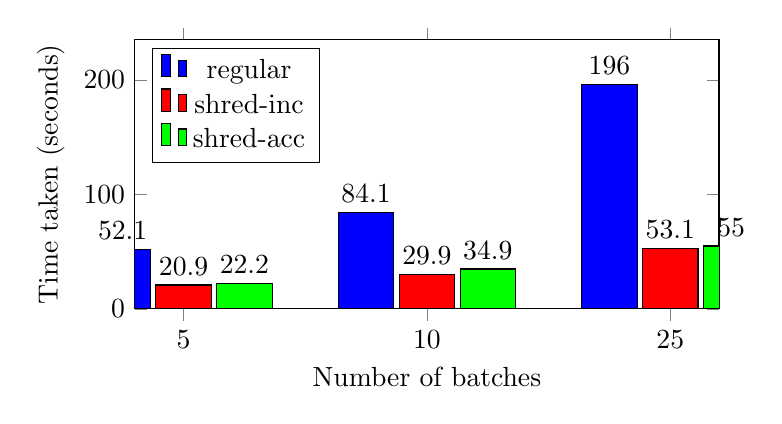
\begin{tikzpicture}
    \begin{axis}[
        ybar,
        ymin=0,
        width  = 9cm,
        height = 5cm,
        bar width=20pt,
        ylabel={Time taken (seconds)},
        xlabel={Number of batches},
        nodes near coords,
 %      nodes near coords align=below, % places labels inside bars
        symbolic x coords={5,10,25},
        xtick = data,
        xtick align=outside,
       enlarge y limits={value=0.2,upper},
        %enlarge x limits={value=0},
        legend pos=north west
    ]
    \addplot[fill=blue] coordinates {(5, 52.1) (10, 84.1) (25, 196)};
    \addplot[fill=red] coordinates {(5, 20.9) (10, 29.9) (25, 53.1)};
    \addplot[fill=green] coordinates {(5, 22.2) (10, 34.9) (25, 55)};
      \legend{regular, shred-inc, shred-acc}
    \end{axis}
\end{tikzpicture}
\end{figure}
}
	



%now enable appendix numbering format and include any appendices
\appendix
\chapter{DSL Codebase} \label{codebase}

\includepdf[pages={1-}]{Expr}
\includepdf[pages={1-}]{Algebra}
\includepdf[pages={1-}]{Eval}
\includepdf[pages={1-}]{ShreddedEval}
\includepdf[pages={1-}]{Streaming}
\includepdf[pages={1-}]{Syntax}
\includepdf[pages={1-}]{Accumulate}
\includepdf[pages={1-}]{Resolver}
\includepdf[pages={1-}]{Tagger}
\includepdf[pages={1-}]{DeepGeneric}

\include{appendix2}

%next line adds the Bibliography to the contents page
\addcontentsline{toc}{chapter}{References}
%uncomment next line to change bibliography name to references
\renewcommand{\bibname}{References}
\bibliography{refs}        %use a bibtex bibliography file refs.bib
\bibliographystyle{plain}  %use the plain bibliography style

\end{document}

